% REMEMBER TO SET LANGUAGE!
\documentclass[a4paper,10pt,english]{article}
\usepackage[utf8]{inputenc}
\usepackage[english]{babel}
% Standard stuff
\usepackage{amsmath,graphicx,varioref,verbatim,amsfonts,geometry, subcaption}
% colors in text
\usepackage{xcolor}
% Hyper refs
\usepackage[colorlinks]{hyperref}

\usepackage[style=phys]{biblatex}

\addbibresource{citations.bib}

% Document formatting
\setlength{\parindent}{0mm}
\setlength{\parskip}{1.5mm}

%Color scheme for listings
\usepackage{textcomp}
\definecolor{listinggray}{gray}{0.9}
\definecolor{lbcolor}{rgb}{0.9,0.9,0.9}

%Listings configuration
\usepackage{listings}
%Hvis du bruker noe annet enn python, endre det her for å få riktig highlighting.
\lstset{
	backgroundcolor=\color{lbcolor},
	tabsize=4,
	rulecolor=,
	language=python,
        basicstyle=\scriptsize,
        upquote=true,
        aboveskip={1.5\baselineskip},
        columns=fixed,
	numbers=left,
        showstringspaces=false,
        extendedchars=true,
        breaklines=true,
        prebreak = \raisebox{0ex}[0ex][0ex]{\ensuremath{\hookleftarrow}},
        frame=single,
        showtabs=false,
        showspaces=false,
        showstringspaces=false,
        identifierstyle=\ttfamily,
        keywordstyle=\color[rgb]{0,0,1},
        commentstyle=\color[rgb]{0.133,0.545,0.133},
        stringstyle=\color[rgb]{0.627,0.126,0.941}
        }
        
\newcounter{subproject}
\renewcommand{\thesubproject}{\alph{subproject}}
\newenvironment{subproj}{
\begin{description}
\item[\refstepcounter{subproject}(\thesubproject)]
}{\end{description}}

%Lettering instead of numbering in different layers
%\renewcommand{\labelenumi}{\alph{enumi}}
%\renewcommand{\thesubsection}{\alph{subsection}}

%opening
\title{Numerical approximation of a multi-dimensional integral using Gaussian quadrature and Monte Carlo methods.}
\author{Caspar William Bruenech}

\begin{document}

\maketitle

\begin{abstract} \centering
    Two versions of both Gaussian quadrature and Monte Carlo methods for approximating a six-dimensional integral were implemented. Results show that Monte Carlo methods featuring importance sampling produced the best accuracy due to its small variance, while also displaying a better scalability for decreasing the error in the result due to the method's independence on the dimensionality of the integral. Nevertheless, for lower dimensional integral, Gaussian quadrature were shown to be a potentially better method, as they converge to a smaller error faster than Monte Carlo. The Monte Carlo algorithm was then parallelized, which, while not producing a speedup equal to the number of CPU cores on the hardware used in this article, displayed a strong feasibility in its implementation
\end{abstract}

\section{Introduction}

The purpose of this experiment is to study various methods of numerical integration. We will be looking at two main methods; Gaussian Quadrature and Monte Carlo, while exploring different variations within these two. The integral we will be studying is a six-dimensional integral originating from quantum mechanics, which will allow us to observe which methods suffer the least from the so-called curse of dimensionality. As the vast majority of integrals do not have an analytical solution, numerical integration is one of the most important tools in modern science. However, as with any numerical calculation, assumptions and approximations are unavoidable, which can cause inaccuracies in the final result. 

\section{Method}

\subsection{The Integral}

The integral in question is the expectation value of the correlation energy between two electrons which repel each other via the Coulomb interaction

\begin{equation} \label{eq:int_cart}
    \langle \frac{1}{|\bold{r}_1 - \bold{r}_2|} \rangle = \int_{-\infty}^\infty \frac{1}{|\bold{r}_1 - \bold{r}_2|} e^{-2\alpha (r_1 + r_2)} d\bold{r}_1 d\bold{r}_2,
\end{equation}

where

$$\bold{r}_i = x_i \bold{e}_x + y_i \bold{e}_y + z_i \bold{e}_z, \qquad r_i =  \sqrt{x_i^2 + y_i^2 + z_i^2},$$

and $\alpha$ is a parameter relating to the charge of the atom in question. We will fix this value to $2$, which corresponds to the charge of the helium atom. This integral has an exact value of $I_{exact} = \frac{5 \pi^2}{16^2}$ which we will use to validate the results of our calculations. Since the integral domain is from $-\infty$ to $\infty$, we need to approximate this value. Due to the integral carrying a negative exponential term, we can plot $e^{-2lambda}$ for increasing values of $\lambda$, and choose a value for $\lambda$ at which the function is $\approx 0$, since the contributed area under the function at higher values than this will be negligible. The result is shown in figure \ref{fig:lambda}, which shows that we only need to be looking at $\lambda \in [2, 6]$ to produce satisfactory results.

\begin{figure}
    \centering
    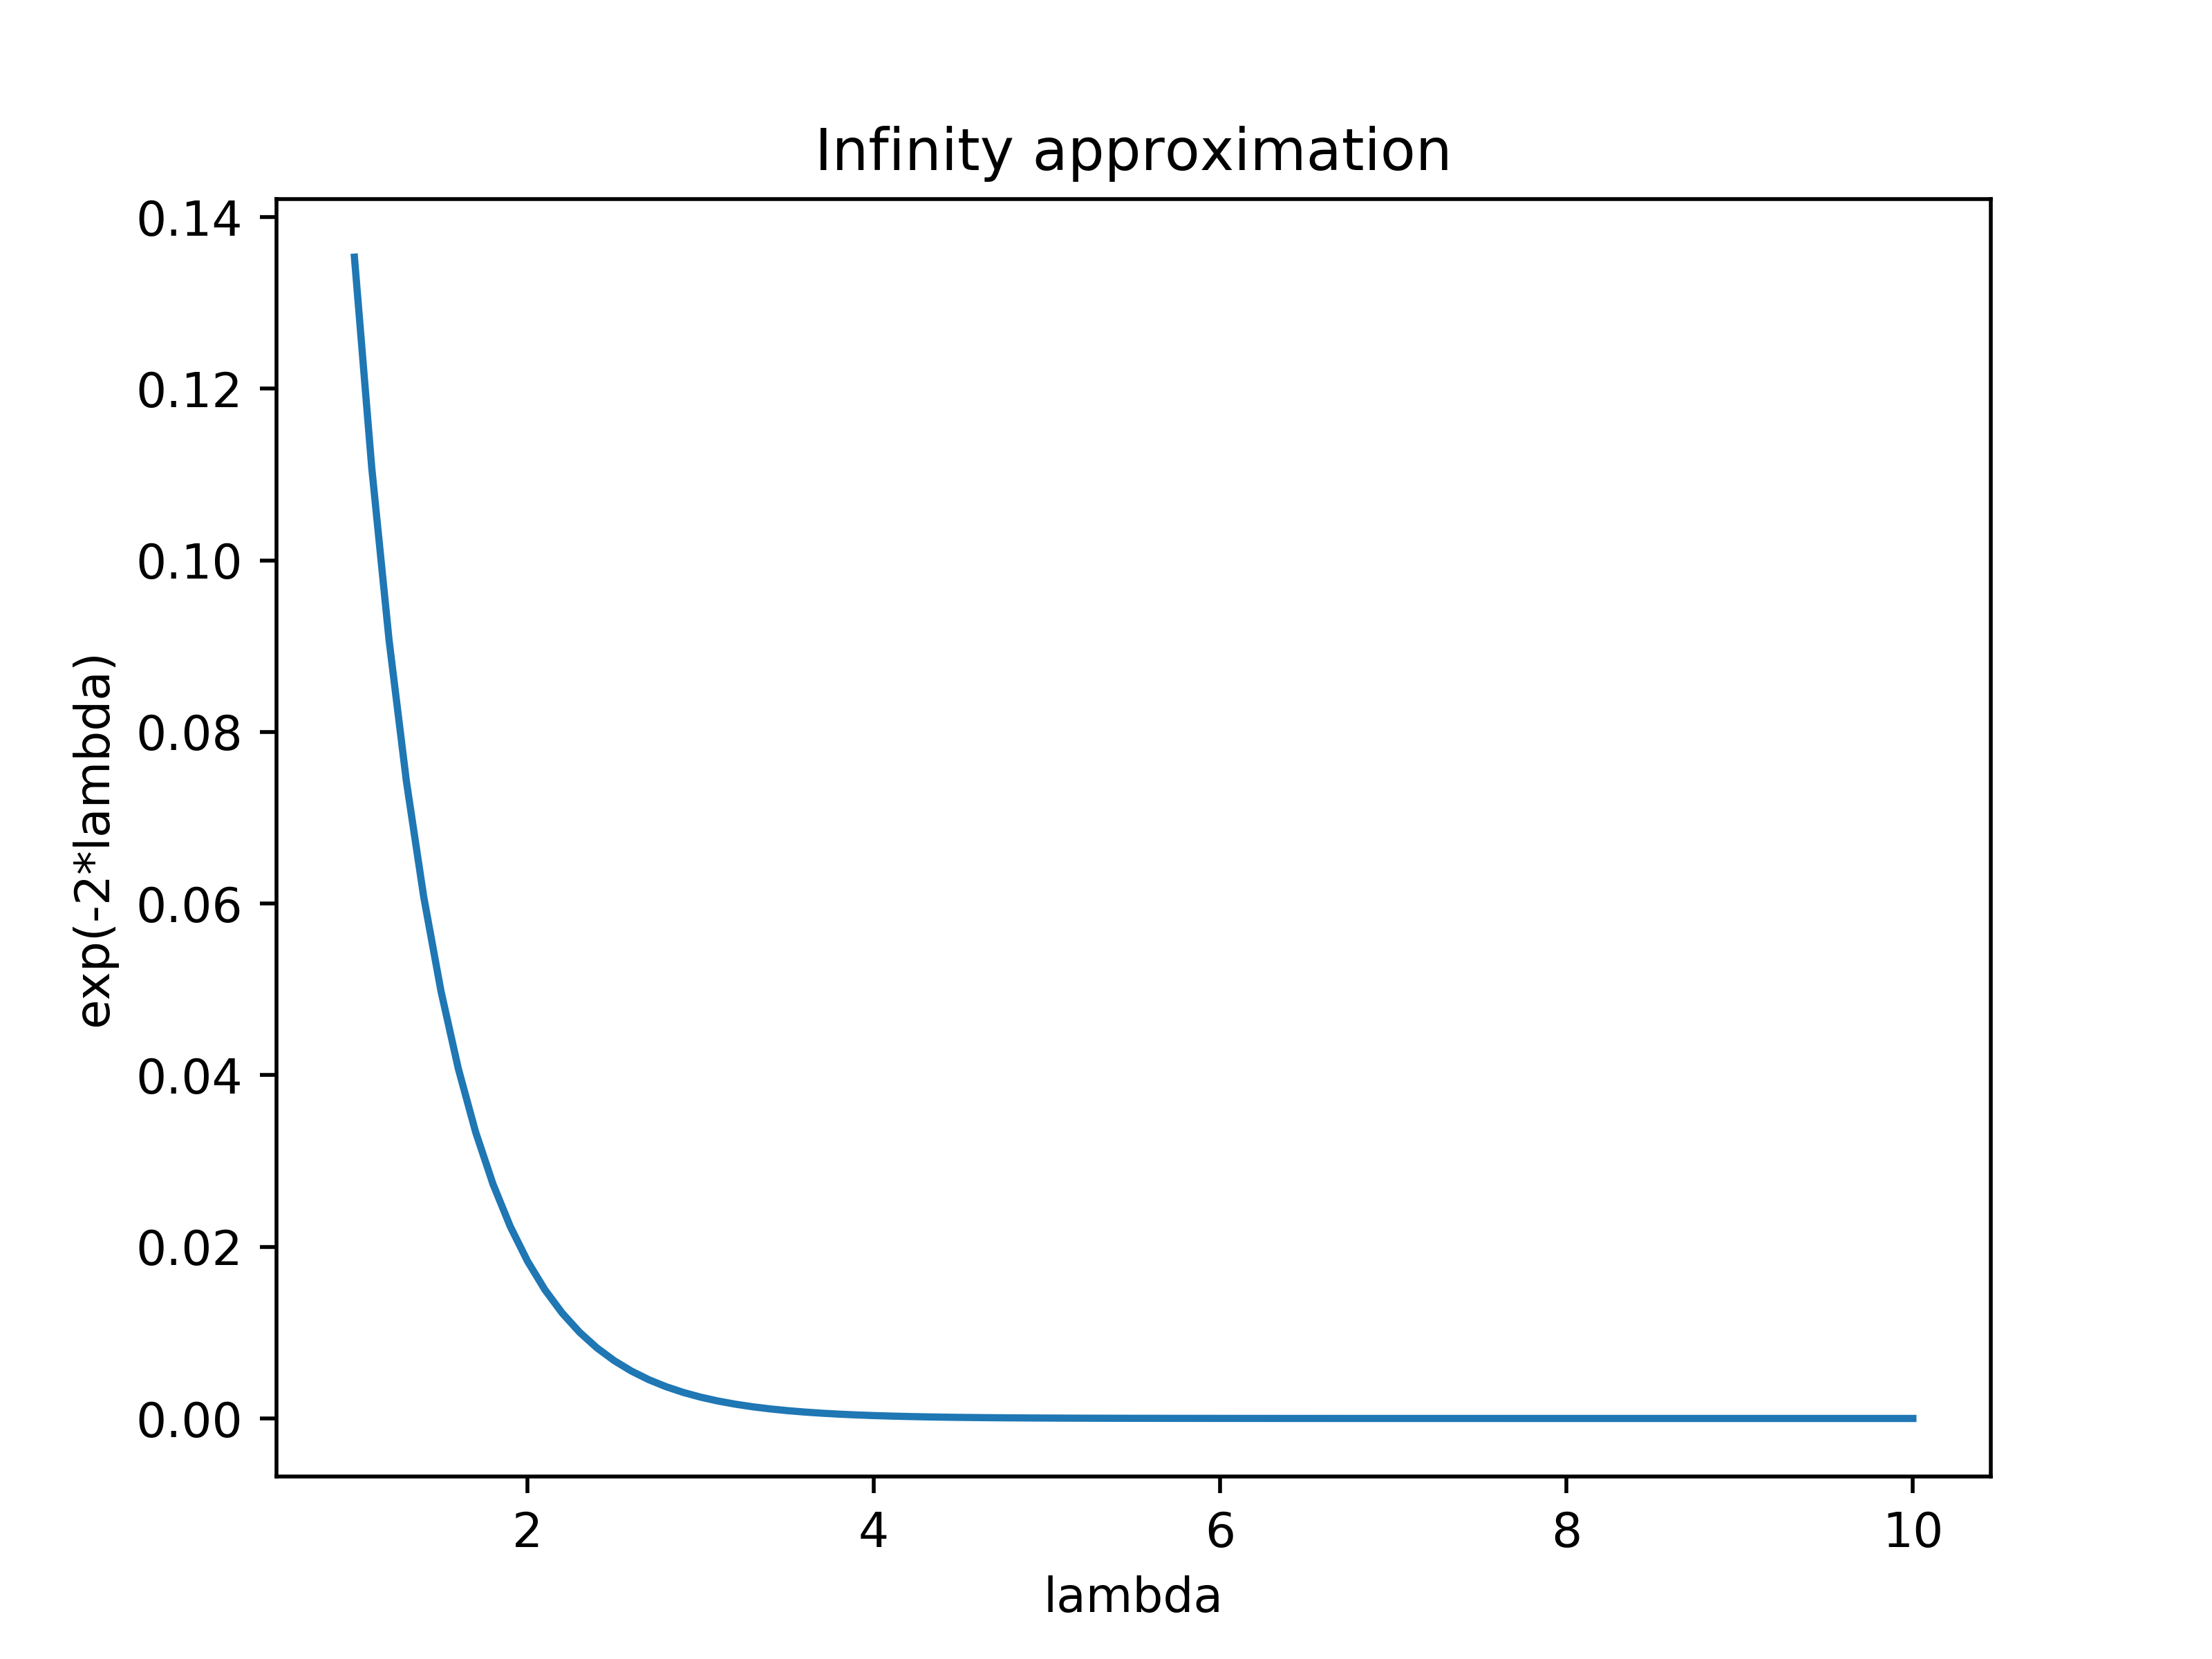
\includegraphics[width=0.4\textwidth]{lambda.png}
    \caption{A plot showing how the function to integrate falls with $\lambda$}
    \label{fig:lambda}
\end{figure}

\subsection{Gaussian Quadrature}

The first method of numerical integration which we will be studying is the method of Gaussian Quadrature. In general, quadrature rules approximates the area under a function as a weighted sum of the function values at specified points. The Gaussian quadrature is a specialized quadrature rule which is designed to produce an exact outcome when applied to polynomials $P$ of degree $2n - 1$ or less. I.e.

$$ \int_a^b P(x) = \sum_{i=1}^n w_i P(x_i)$$

For a function $f$ we then have

$$\int_a^b f(x) \approx \sum_{i=1}^n w_i f(x_i)$$

The idea is then to choose the optimal $x_i$, called abscissas, at which to evaluate the function. The abscissas are the roots of a given orthogonal polynomial, while the weights $w_i$ are defined from a weight function $w(x)$ where

\begin{equation}
    w(x) = \frac{2}{(1 - x^2)[P'_n(x)^]^2}
\end{equation}

Where $P'_n$ is the derivative of the $n$-degree polynomial. Depending on the interval over which do to the integration, different polynomials can be chosen. The two polynomials which we will utilize in this experiment are the Legendre and Laguerre polynomials who, respectively, have the weight functions

$$w(x)^{Leg} = 1, \qquad w(x)^{Lag} = x^{\alpha'} e^{-x}, \quad \alpha' > -1$$

With the Legendre polynomials, the abscissas $x \in [-1, 1]$, while the abscissas produced with Laguerre polynomials have $x \in [0, \infty \rangle$. Since the domain of integration for the integral in question is over $[-\lambda, \lambda]$, we are therefore forced to make a change of limits when using Legendre polynomials. This can be done as

$$\int_a^b f(x) dx = \frac{b - a}{2}\int_{-1}^1 f\left(\frac{b - a}{2}x + \frac{a + b}{2}\right) dx,$$

which means we have to rewrite $x_i$ as

$$x'_i = 2\lambda x_i $$

and multiply the final result by $2\lambda$. Since we, in this case, are dealing with an integral over six dimensions, and all the $x \in [x_1,..,x_6]$ are over the same area ($[-\lambda, \lambda])$, we have to make this change of limits 6 times, and the integral then becomes, using Legendre polynomials;

\begin{equation}\label{eq:spherical_quad}
    I = \langle \frac{1}{|\bold{r_1} - \bold{r_2}|}\rangle \approx (2\lambda)^6 \sum_{i = 1}^N \sum_{j = 1}^N \sum_{k = 1}^N \sum_{l = 1}^N \sum_{m= 1}^N \sum_{n = 1}^N w_i w_j w_k w_l w_m w_n f\left(x'_i, x'_j x'_k, x'_l, x'_m, x'_n\right)
\end{equation} 

where $w$ are the weights calculated from the Legendre polynomial of degree N, and $x'$ are the abscissas with new limits, i.e.

$$x \in [-1, 1] \rightarrow x' \in [-\lambda, \lambda].$$

This is the brute-force implementation of a Gaussian quadrature integral approximation, and will most likely not produce satisfactory results due to the loss of precision when changing the interval of the abscissa (more about this in the discussion). A better approximation might be to rewrite the integral to spherical coordinates. Since this will give us a radial variable $r_i \in [0, \infty\rangle$, we can then apply Laguerre polynomials which are already defined for the same domain, allowing us to avoid having to change the interval of integration, theoretically giving us a better precision and smaller error. By introducing

$$x_i = \rho_i \sin{\theta_i}\cos{\phi_i}$$
$$y_i = \rho_i \sin{\theta_i}\sin{\phi_i}$$
$$z_i = \rho_i \cos{\theta_i}$$

with 

$$r \in [0, \infty\rangle, \quad \theta \in [0, \pi], \quad \phi \in [0, 2\pi \rangle,$$

we can rewrite the integral as

$$I = \int_{-\infty}^\infty dr_1 \int_{-\infty}^\infty dr_2 \int_0^\pi d\theta_1 \int_0^\pi d\theta_2 \int_0^{2\pi} d\phi_1 \int_0^{2\pi} d\phi_2 r_1^2 r_2^2 \sin{\theta_1} \sin{\theta_2} \frac{e^{-2 \alpha (r1 + r2)}}{r_{12}}$$

where

$$r_{12} = \frac{1}{\sqrt{r_1^2 + r_2^2 - 2r_1 r_2 \cos{\beta}}}$$

and 

$$\cos{\beta} = \cos{\theta_1}\cos{\theta_2} + \sin{\theta_1}\sin{\theta_2}\cos{(\phi_1 - \phi_2)}$$

To perform this integral we now need to generate the abscissas and weights for $r_{1,i}$ and $r_{2,i}$ using the Laguerre polynomials, and then use Legendre polynomials to generate the equivalent for $\phi$ and $\theta$. This means we no longer have to make an approximation to infinity, but we do still need to change the limits of the abscissas from the Legendre polynomials for the angles $\theta$ and $\phi$. I.e.

$$x \in [-1, 1] \rightarrow \theta \in [0, \pi] $$

$$x \in [-1, 1] \rightarrow \phi \in [0, 2 \pi]$$

As we saw, the weight function for the Laguerre Polynomials are given by

$$w(x) = x^{\alpha'} e^{-x},$$

where $\alpha'$ is a constant $> -1$.S Since we are using Laguerre polynomials exclusively for the radial part of the integral, the weights becomes

$$w(r_1) = r_1^{\alpha} e^{-r_1} \qquad w(r_2) = r_2^{\alpha} e^{-r_2}$$

We observe that by setting $\alpha = 2$, we can remove the $r_1^2$ and $r_2^2$-terms from our integral, as these values will be included directly in the weights. Additionally, since the integral has the term

$$e^{-4r_1}e^{-4r_2},$$

since $\alpha = 2$, which we can rewrite as

$$e^{-r_1}e^{-3r_2}e^{-r_2}e^{-3r_2} = e^{-r_1}e^{-r_2}e^{-3(r_1 + r_2)},$$

we see that the terms $e^{-r_1}$ and $e_{-r_2}$ will be "baked" into the weights, but we still have to include the term $e^{-3(r_1 + r_2)}$. Finally, due to the necessity og having to change the limits of the abscissas for the $\theta$- and $\phi$-values generated by the Legendre polynomials, we again have to multiply the final result by a factor $(b - a)/2$. Since we, in this case, have to do this for four variables ($\theta_1, \theta_2, \phi_1, \phi_2$), who, respectively, have the limits $[0, \phi] \quad [0, 2\pi )$, the factor becomes

$$\frac{\pi^2}{4} \frac{4\pi^2}{4} = \frac{\pi^4}{4}.$$

Thus, the integral in spherical coordinates can be approximated as



$$I \approx \frac{\pi^4}{4} \sum_{i = 1}^N \sum_{j = 1}^N \sum_{k = 1}^N \sum_{l = 1}^N \sum_{m= 1}^N \sum_{n = 1}^N w^{r_1}_i w^{r_2}_j w^{\theta_1}_k w^{\theta_2}_l w^{\phi_1}_m w^{\phi_2}_n g\left(r_{1,i}, r_{2,j} \theta_{1,k}, \theta_{2,l}, \phi_{1,m}, \phi_{2,m}\right)$$

where the weights and abscissas for the radial variables are generated with Laguerre polynomials, and the equivalent for the angles are generated with Legendre polynomials followed by a change of limits, and 

$$g = \sin_{\theta_1}\sin_{\theta_2}\frac{e^{-3(r_1 + r_2)}}{r_{12}}$$

\subsection{Monte Carlo} \label{sec:mc}

The second group of numerical integration methods we will be looking at are the so-called Monte Carlo methods of integration approximation. Referring to the Monte Carlo Casino in Monaco, these methods rely on repeated random sampling for generating numerical results. In the case of approximating integrals, the idea is to randomly sample variables within the domain of integration, evaluate the function at these values, sum up the resulting function value for a number of iterations, and finally compute the mean of the function values. 

To explain this, we assume we have a set of discrete random values $\bold{\hat{x}} \in {x_1,x_2, ...}$, each with a probability $p_i$. The probability density function (pdf) can then be expressed as 

$$f_\bold{\hat{x}} = \sum_i p_i \delta (x - x_i)$$

where $\delta$ is the Dirac-delta function. We then assume we perform an experiment whose outcome we denote $\xi$. The random variable $\bold{\hat{x}}$ then assigns a real number \bold{\hat{x}}(\ksi) to this experiment result, which means we can use a real function $G(x)$ to define a new random variable $\bold{\hat{G}}$ where $\bold{\hat{G(\xi)}} = G(\bold{\hat{x}}(\xi))$. For random variables with a pdf $f_\bold{\hat{x}}$, the expectation value of this new random variable \bold{\hat{G}} is then

$$\mathbb{E} = \int_{\infty}^\infty f_\bold{\hat{x}}G(x)$$

With this in mind, let us assume we want to calculate the integral

$$I = \int_a^b g(x) dx$$

We can rewrite the integral as

$$I = \int G(x) f_\bold{\hat{x}}(x) dx$$

Which we recognize as the expectation value (average value) of $G(x)$ with respect to the random variable $\bold{\hat{x}}$ with the pdf $f_\bold{\hat{x}}$. I.e. $I = \mathbb{G}$. This means that, by performing $N$ experiments such that we generate $N$ random values $x_i$, the sample mean and sample variance can be calculated as

$$\overline{\mu} = \frac{1}{N} \sum_{i=1}^N G(x_i)$$

$$\overline{\sigma^2} = \frac{1}{N} \sum_{i = 1}^N G(x_i)^2 - \left( \frac{1}{N} \sum_{i = 1}^N G(x_i) \right)^2. $$

It can be shown, by using Chebyshev's theorem \cite{Toral+Colet}, that the true mean value $\mu$ and variance $\sigma^2$ of the experiment can be estimated as

\begin{equation} \label{eq:mu_samp}
    \mu = \overline{\mu} \pm \frac{\overline{\sigma}}{\sqrt{N}}
\end{equation}

\begin{equation}\label{eq:sigma_samp}
    \sigma = \overline{\sigma} \pm \frac{\overline{\sigma}}{\sqrt{2N}} 
\end{equation}


Which shows that the error of the estimation of these values goes to zero as the number of repeated experiments $N \rightarrow \infty$. This is known as the \textit{central limit theorem}. This means that our integral can now be written as

$$I = \overline{\mu} \pm \frac{\overline{\sigma}}{\sqrt{N}} \approx \overline{\mu}.$$

Where $\overline{\mu}$ and $\overline{\sigma}$ are calculated, respectively, from equation \ref{eq:mu_samp} and \ref{eq:sigma_samp}, and 
$$G(x) = \frac{g(x)}{f_\bold{\hat{x}}(x)}.$$

where $g(x)$ is the function we want to integrate, and $f_\bold{\hat{x}}(x)$ is the probability distribution function for the random variables $\bold{\hat{x}}$. 


We will be performing Monte Carlo integral approximation in two ways; (1) by randomly sampling $\bold{x}$-values in the domain $[0, 1]$ and mapping to $[-\lambda, \lambda]$ using a uniform probability distribution given by

\[ {f_\bold{\hat{x}}(x)} = \begin{cases} 
1, \quad x \in [-1, 1] \\
0, \quad \textit{else},
\end{cases} \]

and evaluating \ref{eq:int_cart} at these values, and (2), by using an exponential probability distribution such that 

\[ {f_\bold{\hat{x}}(x)} = \begin{cases} 
\lambda a^{-\lambda x}, \quad x \geq 0 \\
0, \quad \textit{else}, 
\end{cases} \]

an applying this to the function in spherical coordinates. The reason for using two different methods is to observe how the choice of a suitable pdf can (hopefully) improve the results of the integral we want to approximate. This is called importance sampling. We know that the function we want to integrate behaves similar to the plot in figure \ref{fig:lambda}. This means that when we sample \textit{uniformly} distributed random variables in the interval $[-\lambda, \lambda]$ (after mapping), we see that we will very likely generate multiple variables which do not fall under the function. As the function goes to $\infty$ when $x \rightarrow 0$, we could either choose $\lambda$ such that we encompass the majority of the area under the function (this would be equivalent to for example $\lambda = \pm 4$ in figure \ref{fig:lambda}), however, since they are uniformly distributed, we will be generating values that do not fall in this area, forcing to have to perform more iterations in order to get a good approximation of the value of the area (integral). A way to get around this issue, is to choose a probability density function which closely follows the function we want to integrate. Knowing that our function goes as $\exp(-x)$, a good choice for a pdf is the exponential distribution which is defined for $[0, \infty \rangle$, meaning that if we implement this for the radial part of the function in spherical coordinates, we do not have to approximate $\infty$. Figure \ref{fig:uni_v_expo} shows histograms of samples generated with both uniform and exponential distributions. As expected, we see that the exponential distribution closely follows our function, which means that most of the random parameters generated with this pdf will land in the interval with the largest contribution to the total area defined by the function.  This should allow us to get a better approximation to the integral with fewer iterations, compared to with the uniform distribution.

\begin{figure}
    \centering
    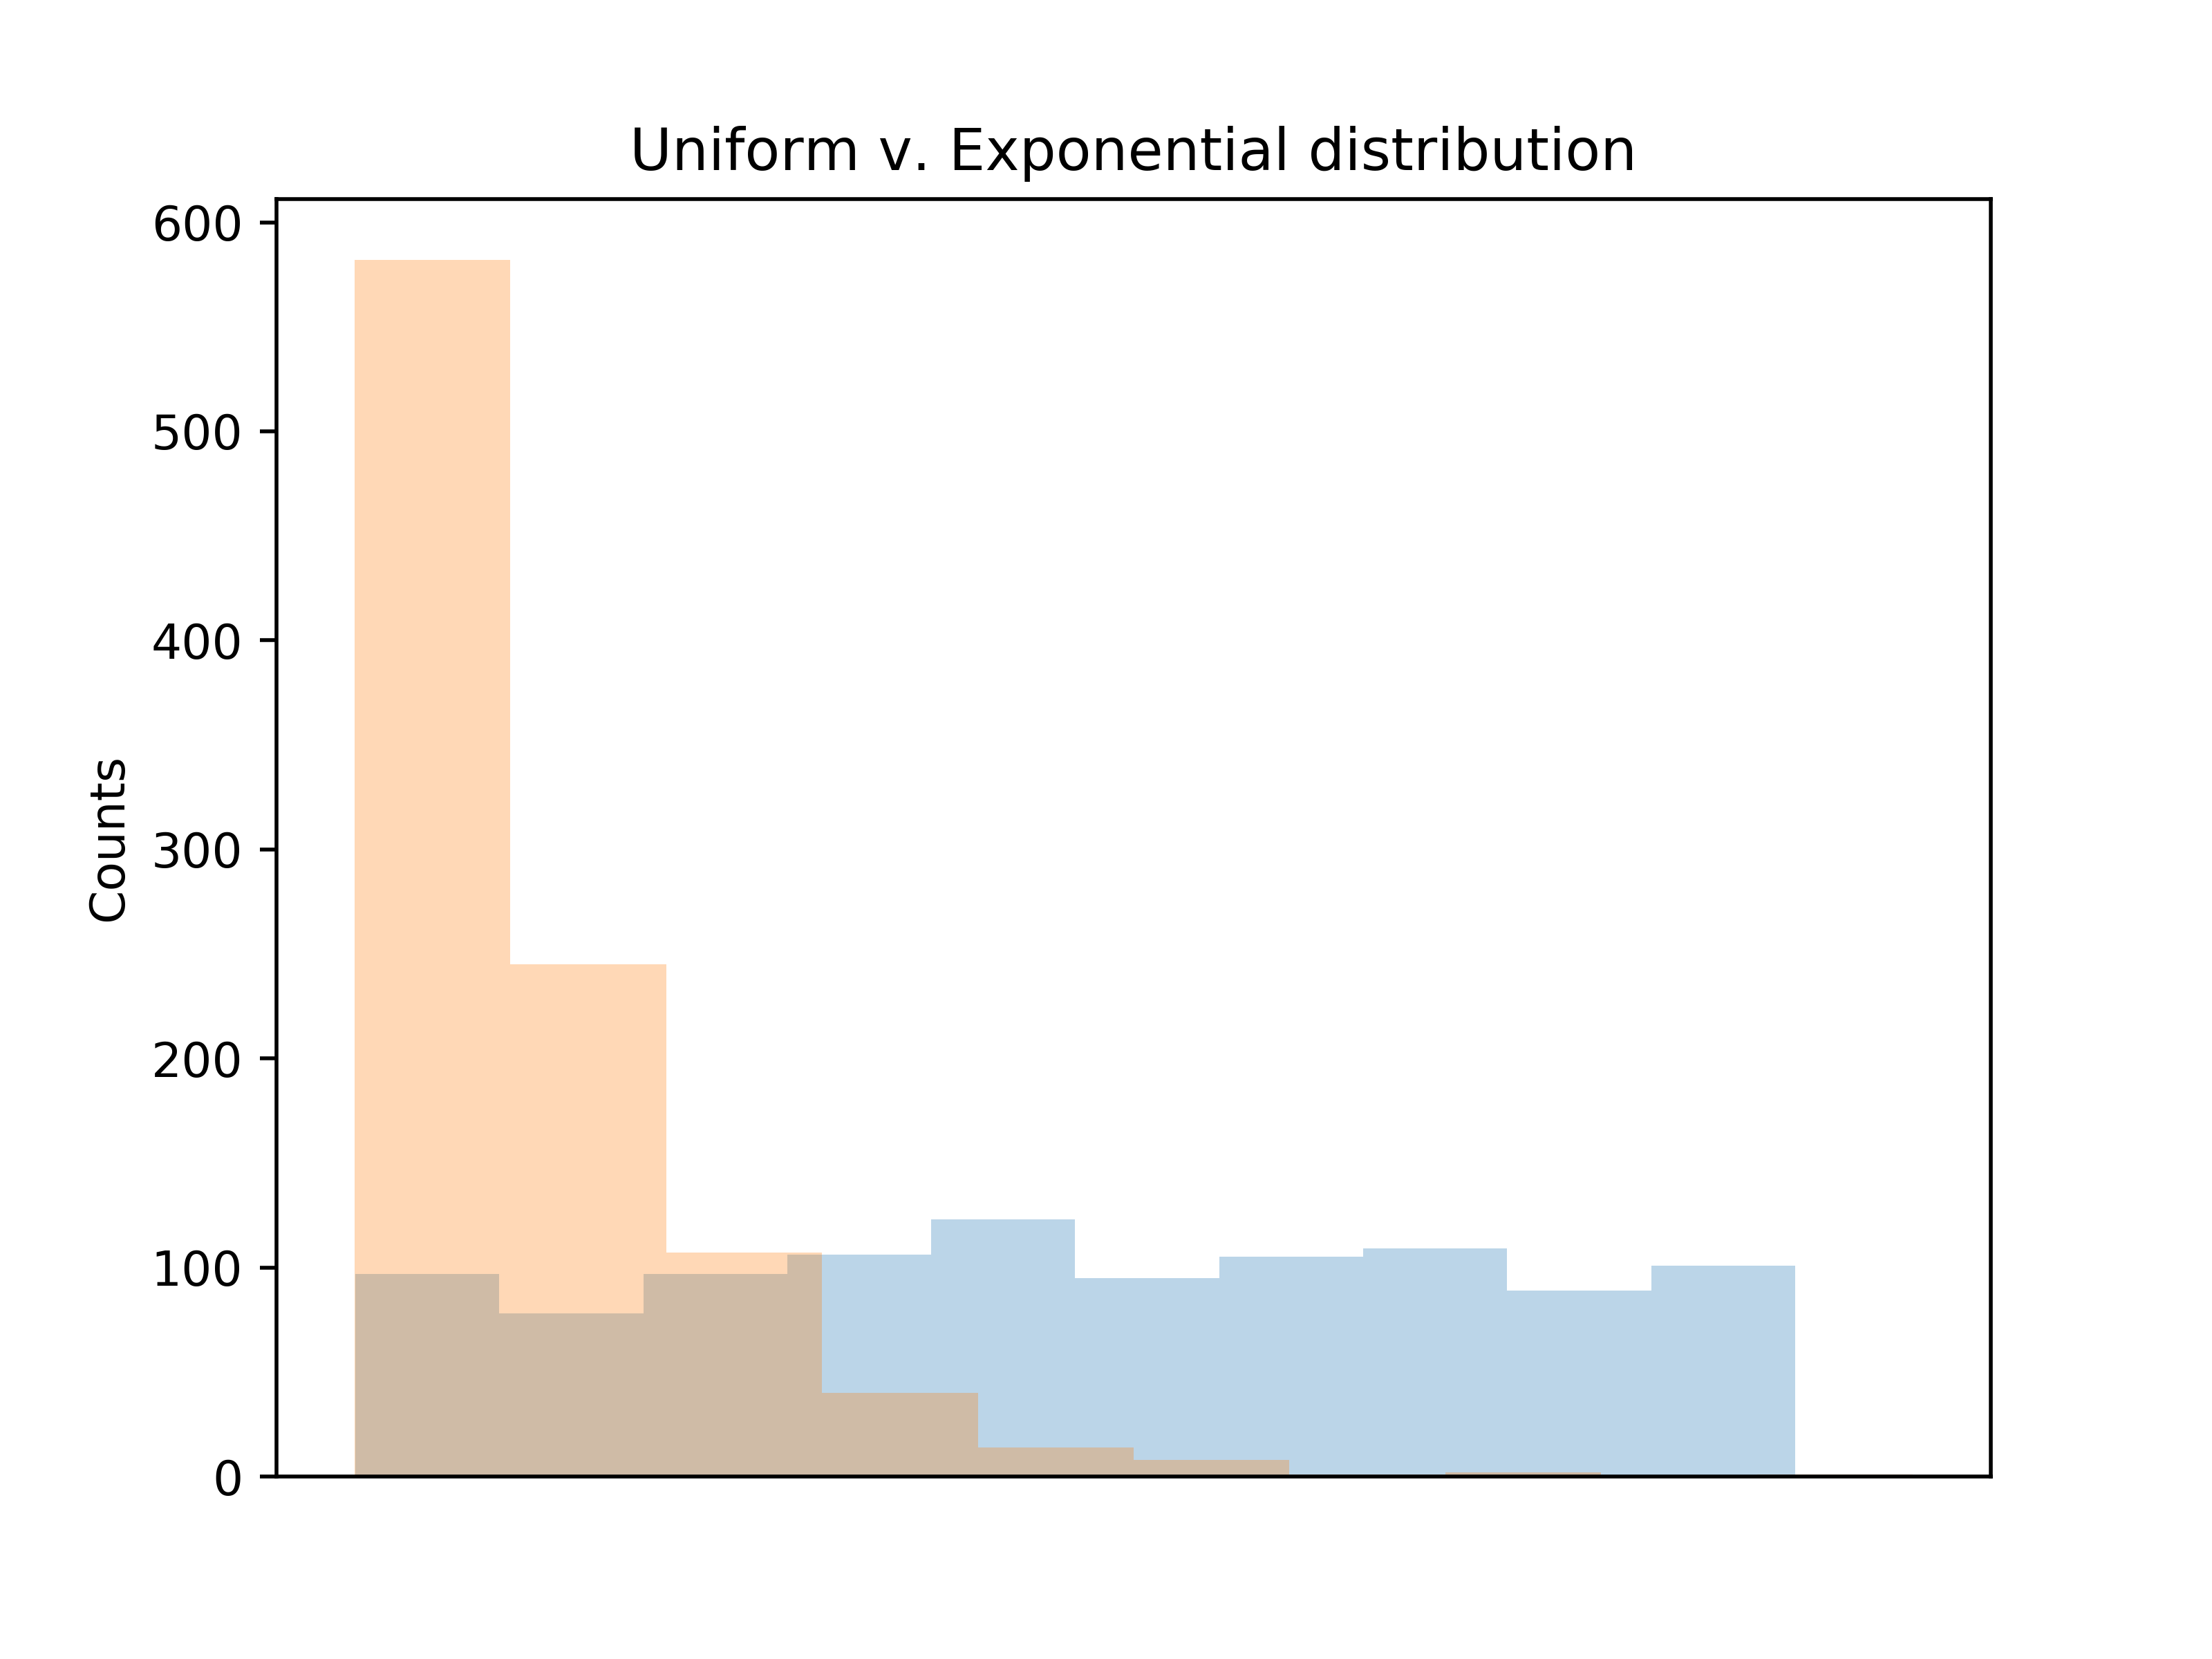
\includegraphics[width=0.5\textwidth]{uni_v_expo.png}
    \caption{A figure showing the distribution of numbers generated by uniform and exponential distributions.}
    \label{fig:uni_v_expo}
\end{figure}


For the case of uniform distribution, we will perform $N$ experiments, with each experiment consisting of

\begin{itemize}
    \item Generating 6 random, uniformly distributed variables $\bold{x} \in [0, 1]$ where $\bold{x} = [x_1, x_2, ..., x_6]$, representing $x_1, y_1, z_1, x_2, y_2, z_2$.
    \item Mapping each variable such that $\bold{x}' \in [-\lambda, \lambda]$, where $\lambda$ is the given approximation to infinity, via the transformation $\bold{x}' = -\lambda + 2\lambda \times \bold{x}$
    \item Evaluating the function at the new variables $\bold{x}'$, such that $y = f(\bold{x}')$
    \item Summing the result and the square of the result in two separate variables
\end{itemize}

The two sums ($y$ and $y^2$), are then divided by $N$ to get the mean sample value, before multiplying by $(2\lambda)^6$ due to the mapping. Finally, the sample standard deviation is calculated from \ref{eq:sigma_samp}.

For the exponential distribution, a similar method will be adopted. Note that we will only be sampling the radial parameters with an exponential distribution, as the exponential term is only dependent on these. The angles will be sampled from a uniform distribution and mapped to their appropriate values, similar to the brute force implementation. Since the exponential terms goes as $exp(-4(r_1 + r_2))$, the probability distribution function will be given as

$$f(r) = 4 e^{-4r}.$$

In order to perform the mapping, we will first generate uniformly distributed values between $0$ and $1$. Assuming that the probability is conserved, we then have the relation

$$p(y) dy = p(x) dx$$

where $y$ are the new values which we want after mapping $x$, $p(y)$ is the exponential pdf as described above, and $p(x)$ is the uniform pdf, which as we know is equal to $1$. This then gives us

$$4e^{-4y} = dx$$

Integrating from $0$ to $y$ we get

$$x = 4\int_0^y e^{-4y} dy = 1 - e^{-4y}$$

Which gives us our mapping from $x \in [0, 1]$ to $y \in [0, \infty\rangle$ as 

\begin{equation}\label{eq:expo_map}
    y(x) = -\frac{1}{4}(1 - x).
\end{equation} 

The implementation of the Monte Carlo integration approximation with importance sampling is then

\begin{itemize}
    \item Generate 6 random, uniformly distributed variables $\bold{x} \in [0, 1]$
    \item Map $x_1$ and $x_2$ to $[0, \infty \rangle$ using \ref{eq:expo_map}, which will be equivalent to $r_1$ and $r_2$.
    \item Map the angular parameters to their corresponding domain my multiplying the remaining four $x$-values by $\pi$ and $2\pi$ for, respectively, $\theta$ and $\phi$. 
    \item Evaluate the function in spherical coordinates with the mapped parameters, divided by the product of the probability distribution evaluated at $r_1$ and $r_2$, such that we get $G(x)$.
    \item Sum the results
\end{itemize}

The remaining procedure is then equivalent to the brute force implementation, except we have to multiply with $4\pi^4$, as a result of changing the limits for the angular parameters.

\subsection{Parallelization}

As Monte Carlo integration usually requires billions of iterations in order to produce satisfactory results, combined with each iteration being independent of one another, makes Monte Carlo simulations a perfect candidate for parallelization.

\section{Implementation}

Note: this article has defined error as the relative error between the computed result and the analytical solution, i.e,

$$error = \frac{|I_{est} - I_{exact}|}{I_{est}}$$

\subsection{Gaussian quadrature results}

Gaussian quadrature using Legendre polynomials was implemented using the integral approximated as defined by \ref{eq:spherical_quad}. The weights and abscissas for both Legendre and Laguerre polynomials were calculated for the N-point integration using the \textit{GaussQuadrature.jl}-module for the Julia programming language\footnote{\url{https://github.com/billmclean/GaussQuadrature.jl}}. The integral was computed for $N \in [2, 30]$, and $\lambda \in [1, 6]$. The result of this is shown in figure \ref{fig:legendre_all}.  Upon observing that the results were better (the error was lower) for odd values of $N$, the experiments were repeated, this time for only the odd values of $N \in {3, 29}$. The result of this is shown in the heat map in figure \ref{fig:legendre_odd}. 

\begin{figure}[h!]
  \centering
  \begin{subfigure}[b]{0.45\linewidth}
    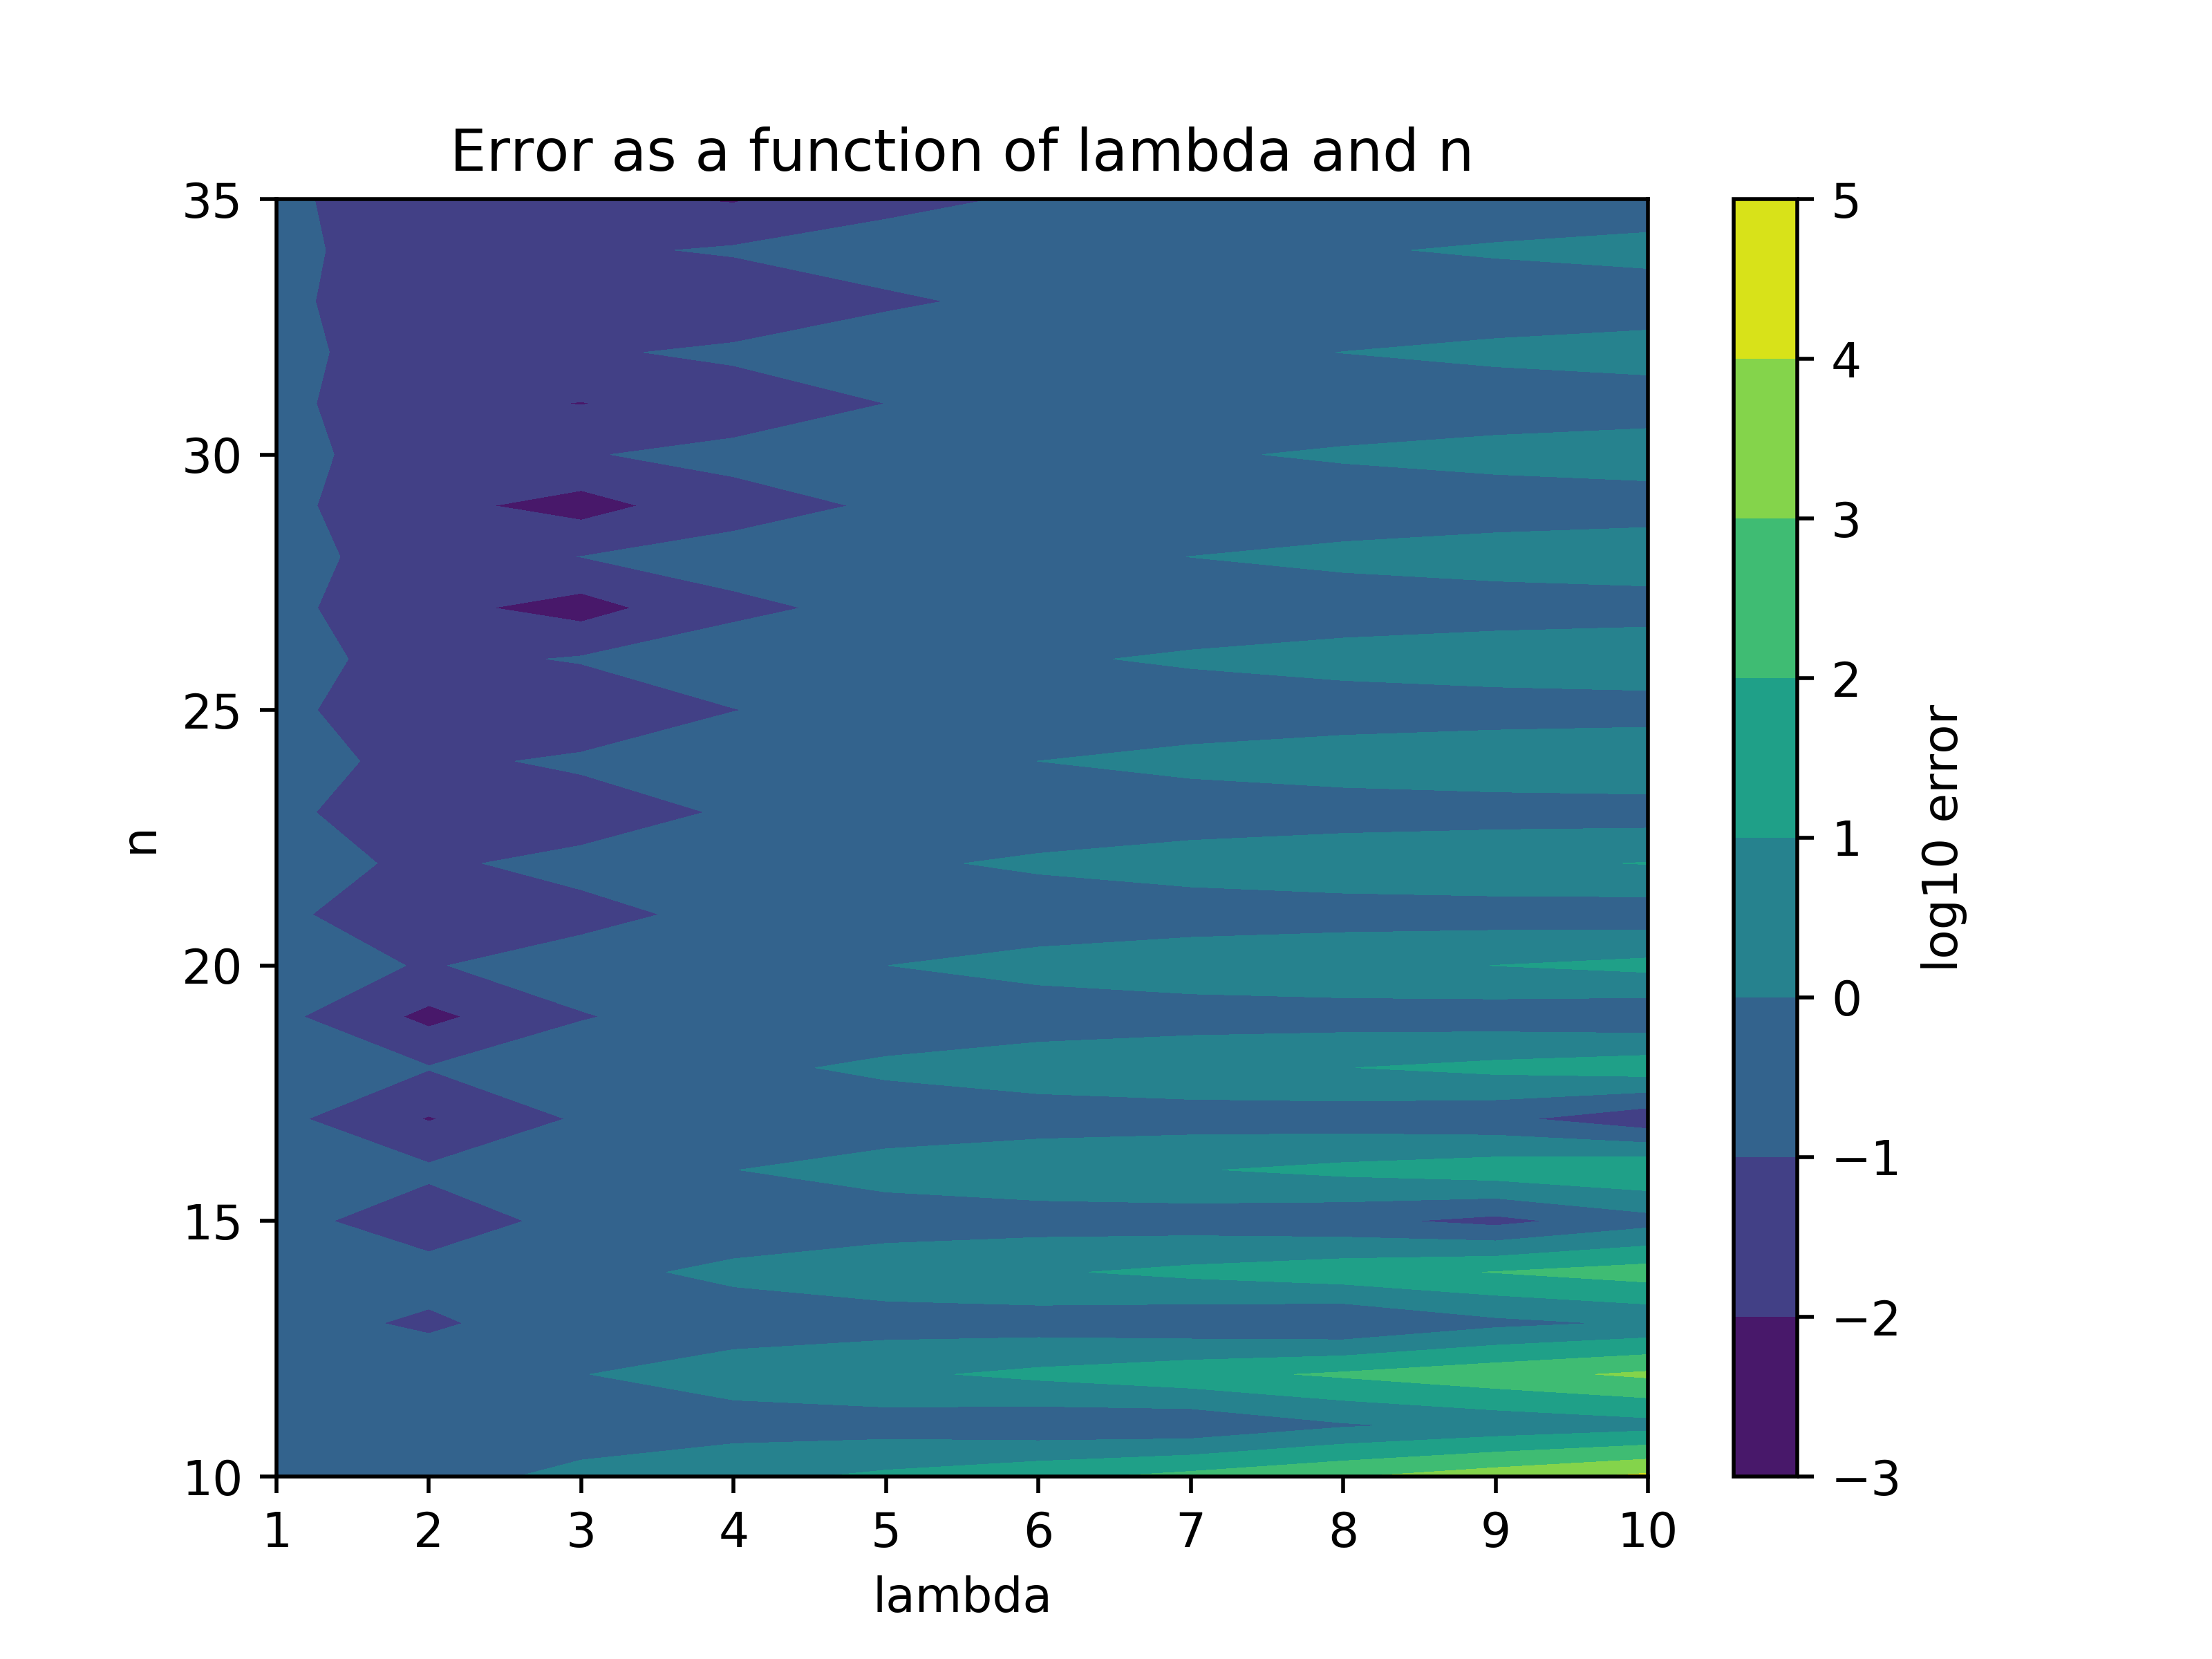
\includegraphics[width=\linewidth]{legendre_error.png}
    \caption{A contour plot of the error produced by the integral approximation using Legendre polynomials, as a function of the polynomial degree N and the infinity approximation $\lambda$.}
    \label{fig:legendre_all}
  \end{subfigure}
  \begin{subfigure}[b]{0.45\linewidth}
    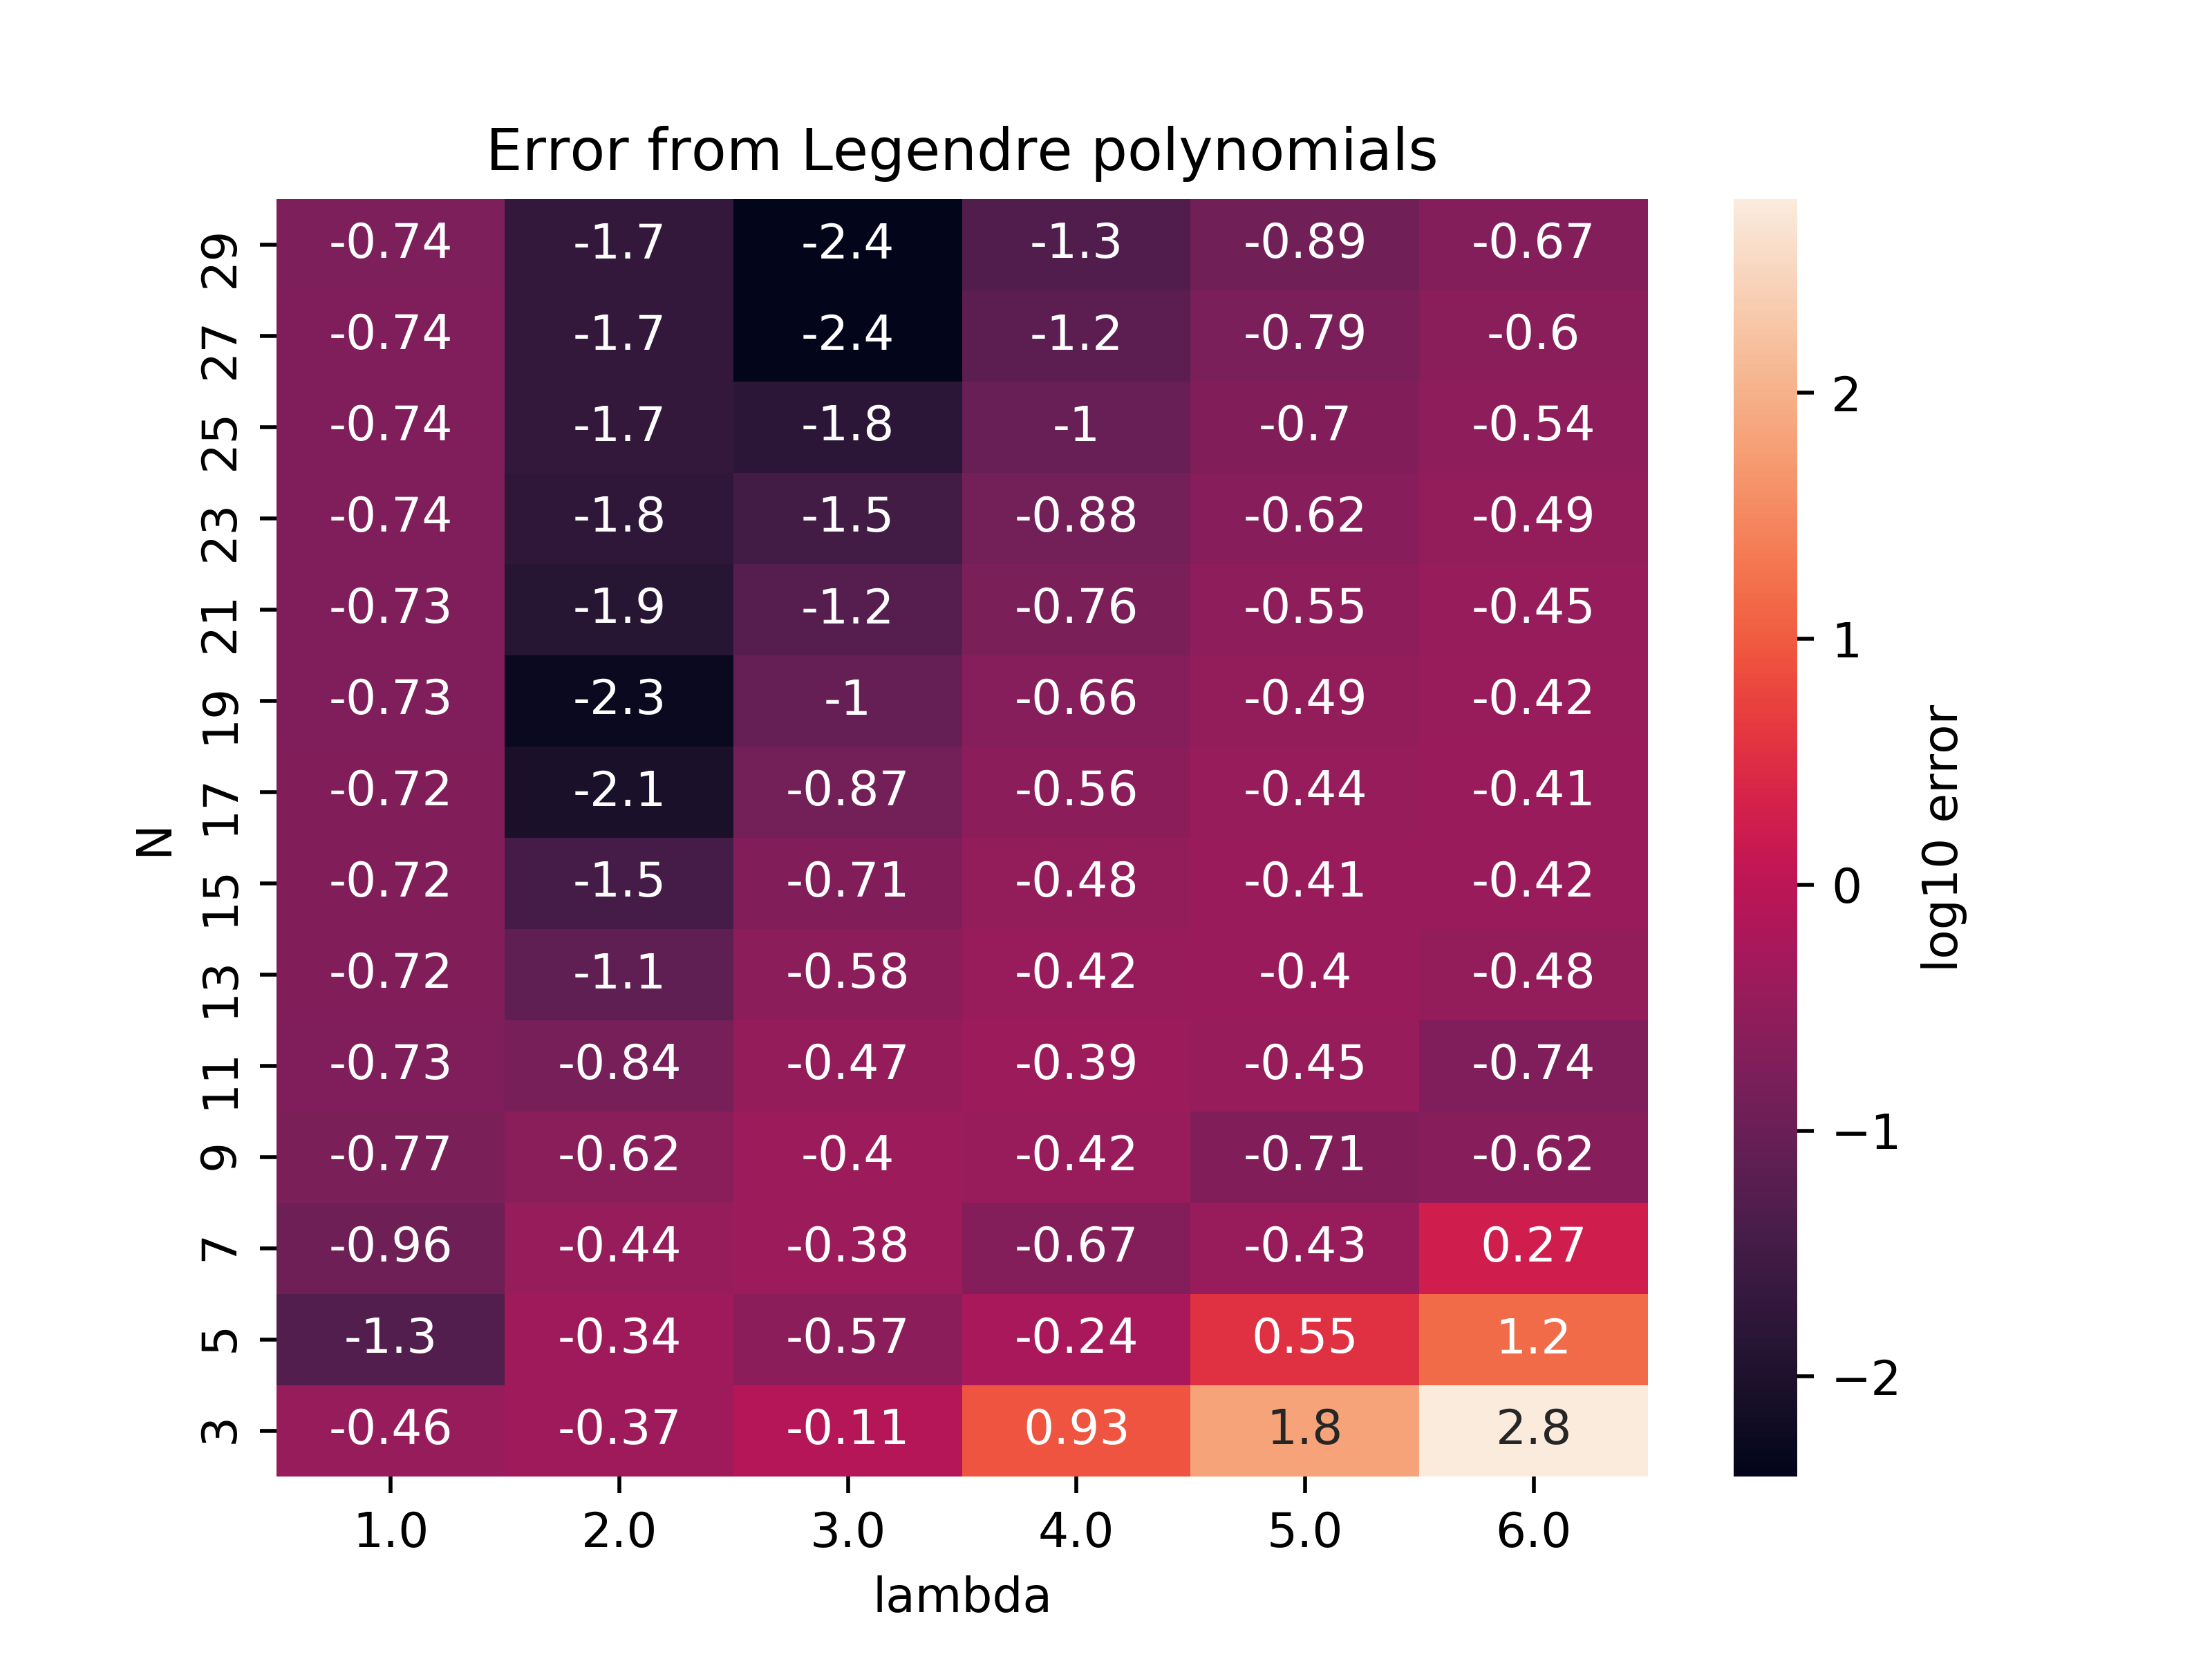
\includegraphics[width=\linewidth]{legendre_heatmap.png}
    \caption{A heat map of the same error, this time with a smaller selection of n's and $\lambda$}
    \label{fig:legendre_odd}
  \end{subfigure}
 
\end{figure}

The integral approximation was then implemented using Laguerre polynomials and evaluated for the same $N$-values. The results were plotted and compared to the results from the Legendre polynomials with $\lambda = 3$, as this value of $\lambda$ produced the smallest error with the Legendre implementation. This result is shown in figure \ref{fig:laguerre_legendre}. The figure includes the resulting value of the approximated integral compared to the exact analytical solution, the error produced by both methods, and a log-log plot of the CPU time taken vs. the polynomial degree. 


\begin{figure}
    \centering
    \textbf{Gaussian Quadrature results}\par\medskip

    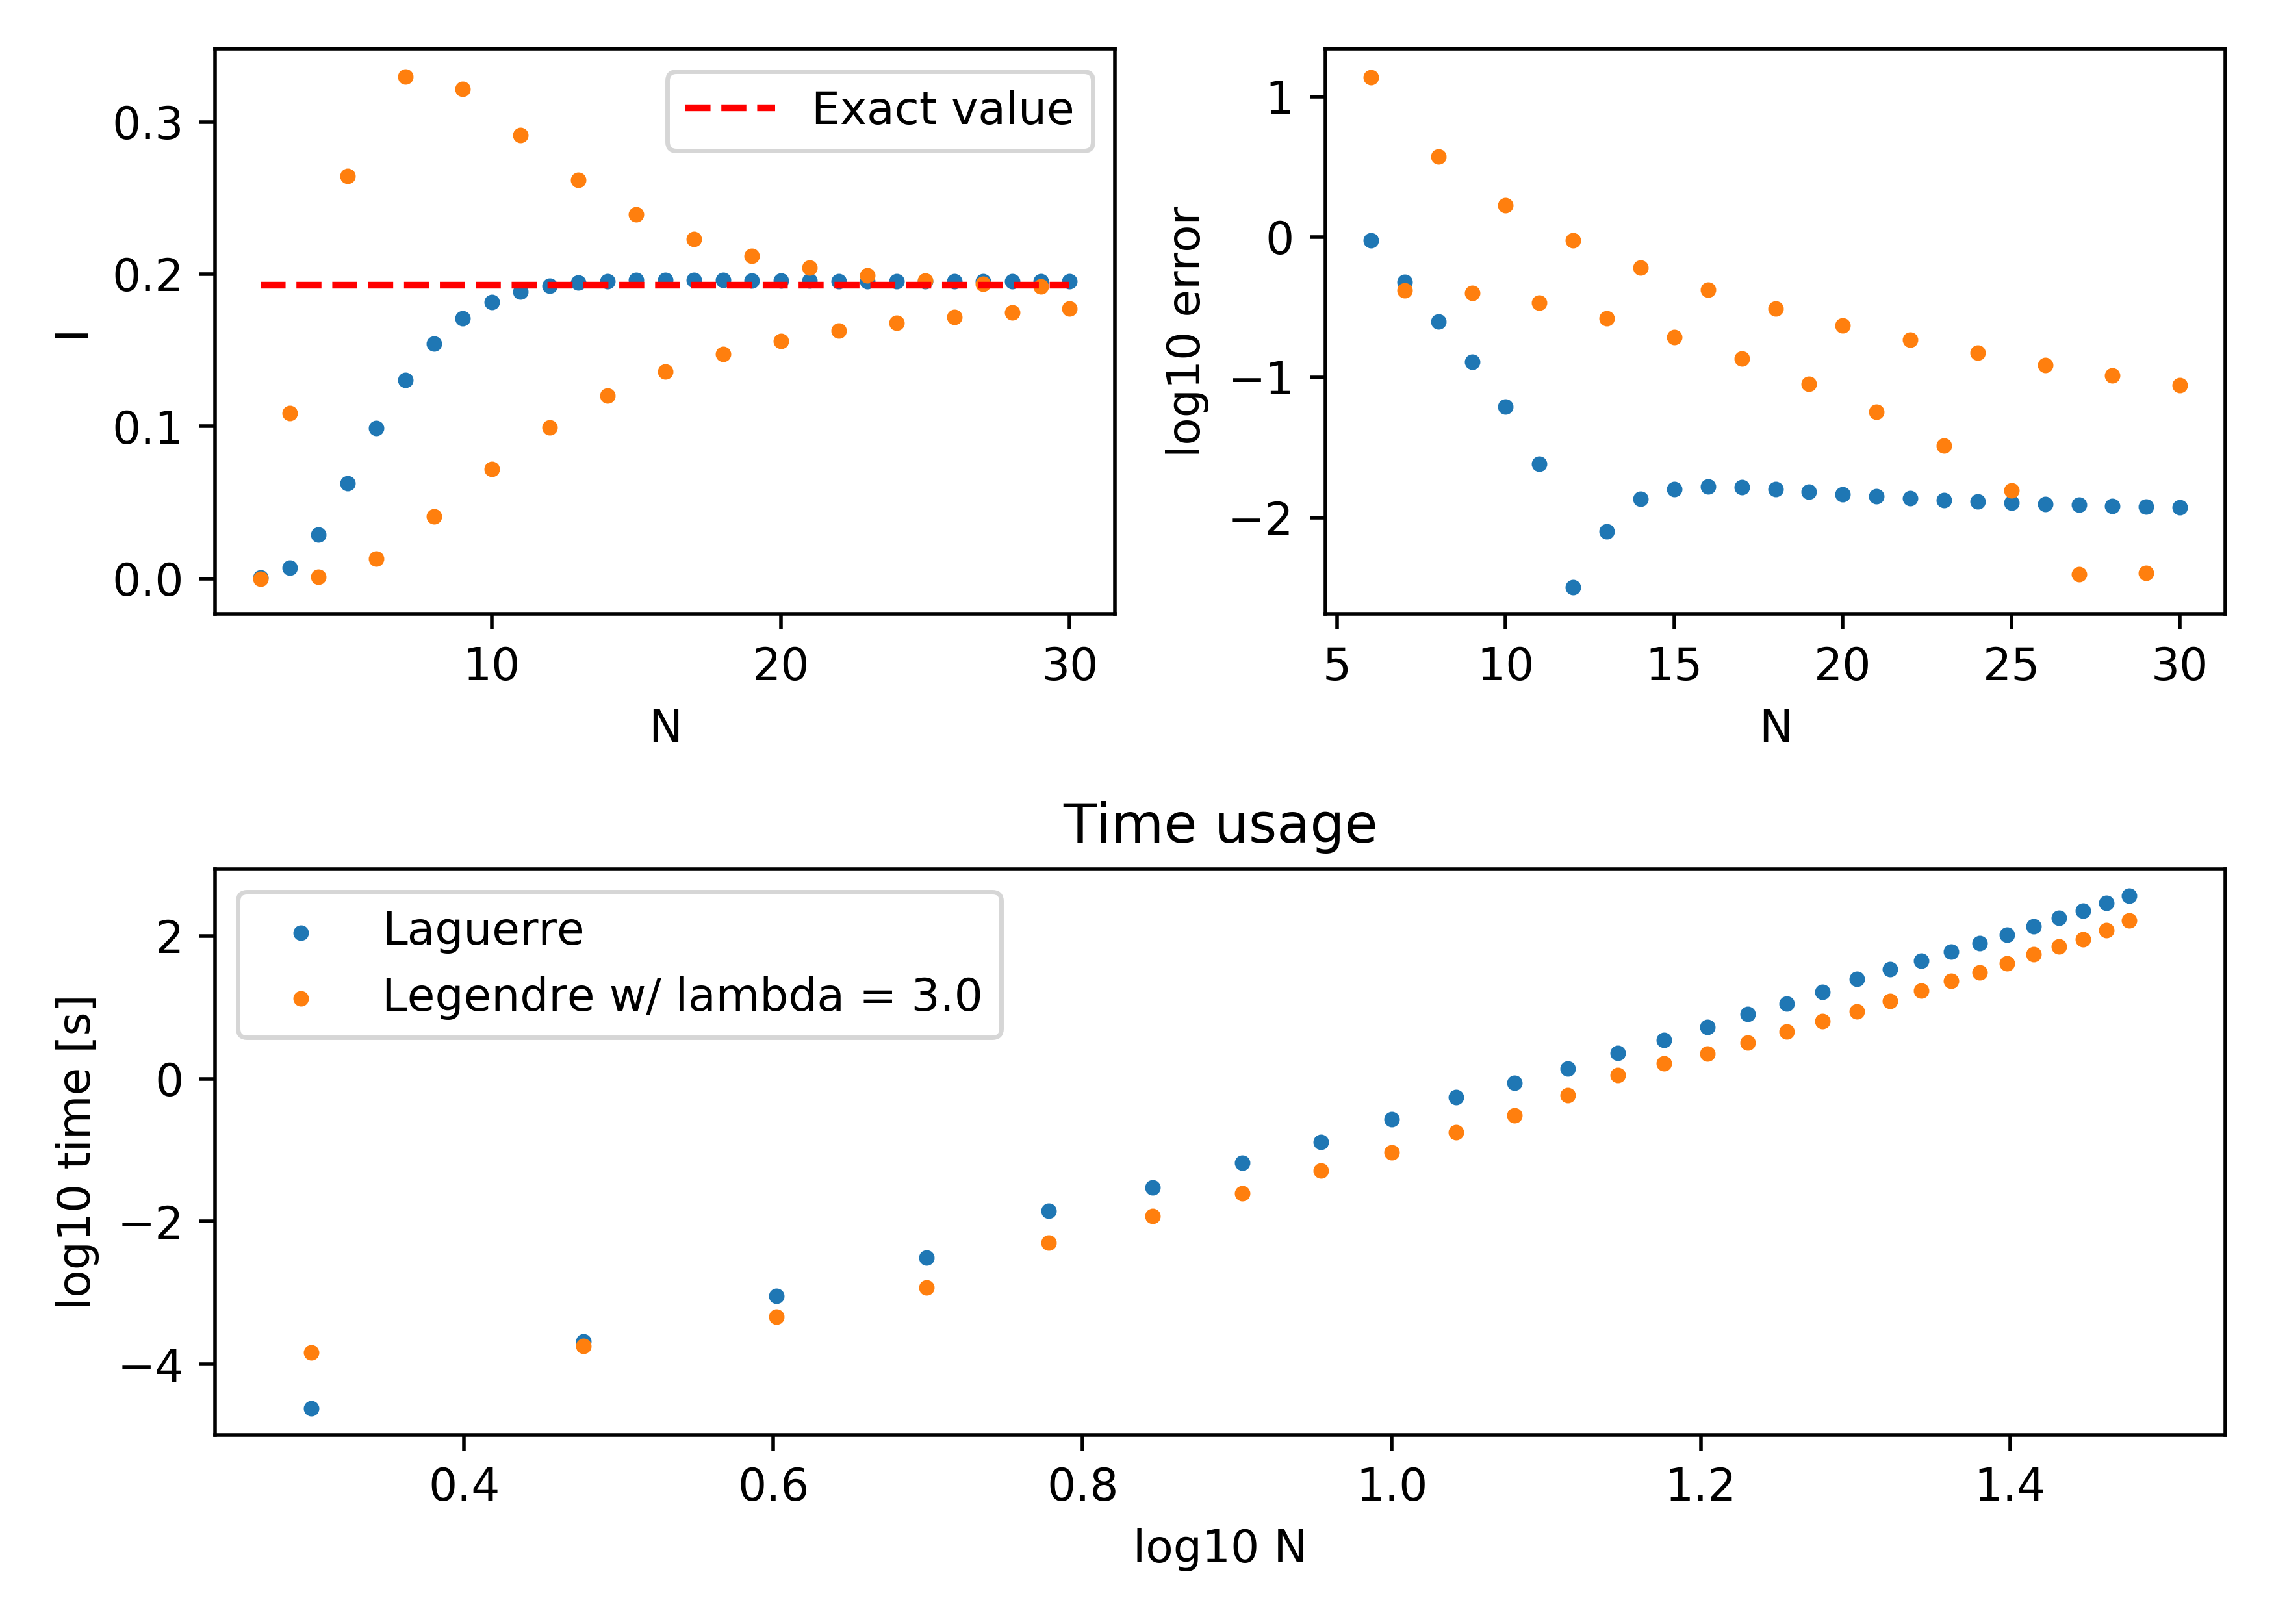
\includegraphics[width=\textwidth]{laguerre_legendre.png}
    \caption{Figures showing the results of the integral approximation using Laguerre and Legendre polynomials with varying polynomial degrees. All the results from the Legendre polynomials were calculated with $\lambda=3$. The top row shows, respectively, the result of the integral approximation with both methods, with the red line indicating the exact analytical solution to the integral, followed by the $log_{10}$ of the error produced. Finally, the bottom row displays a log-log plot of the CPU time taken by both methods for the same values of $N$.}
    \label{fig:laguerre_legendre}
\end{figure}

\subsection{Monte Carlo results}\label{sec:mc_res}


Monte Carlo integration with and without importance sampling was implemented as described in \ref{sec:mc}. The algorithms were run for $log_{10}(n) \in {1, 8}$ iterations, with the infinity approximation $\lambda = 3$ for the brute-force method. For each value of $n$, 100 experiments were run and the error, standard deviation, and CPU time usage was documented for each experiment. The mean of the error and CPU time for all 100 experiments was calculated for each $n$. Since the standard deviation is not linear, and therefore not additive, the same approach was not possible for this quantity. However, the variance is an additive quantity, allowing the mean of the standard deviation over all experiment runs to be calculated by squaring the standard deviations, calculating their means, and then taking the square root. A plot of these results is shown in figure \ref{fig:montecarlo}. Finally, the result of 100 experiments, each with $n=10^8$ iterations was plotted for both the brute force and the improved method. This is shown in figure \ref{fig:100_exps}.

\begin{figure}
    \centering
    \textbf{Monte Carlo simulation results}\par\medskip

    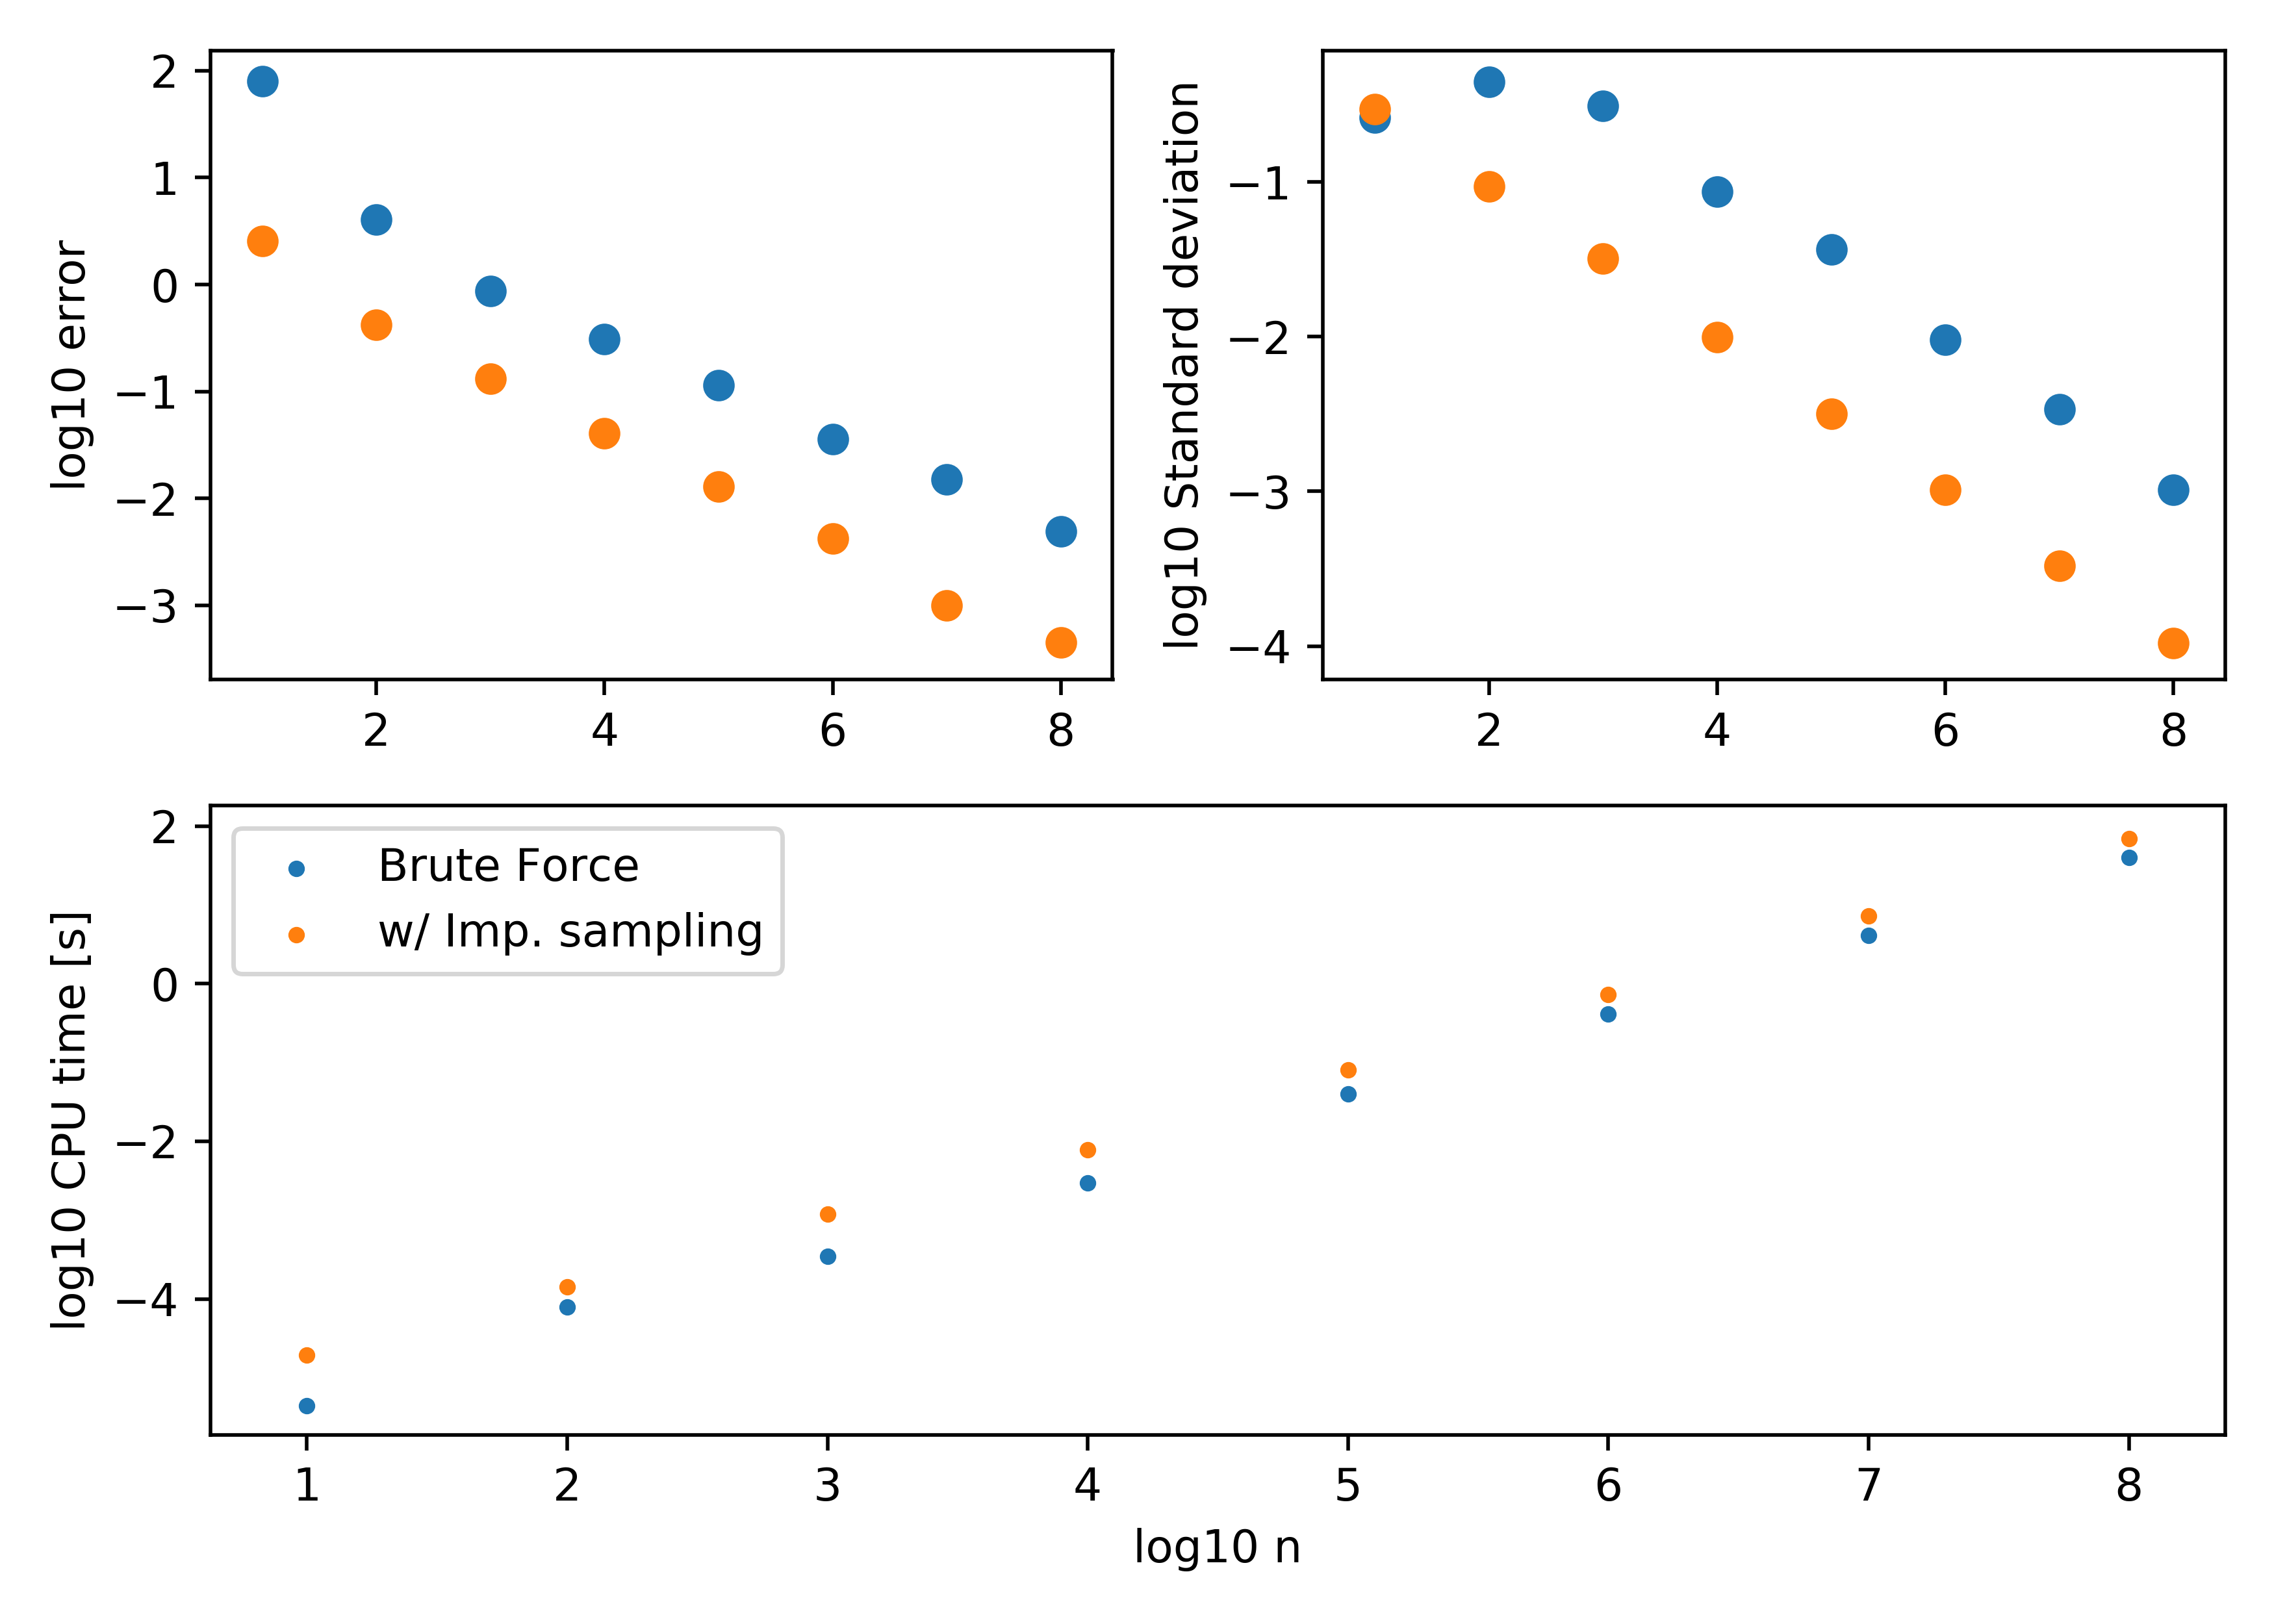
\includegraphics[width=\textwidth]{montecarlo.png}
    \caption{Three plots showing the mean results of Monte Carlo simulations. For each value of $n$, the error, std. dev., and CPU time was measured 100 times. The brute force implementation was used with $\lambda = 3$.}
    \label{fig:montecarlo}
\end{figure}

\begin{figure}
    \centering
    \textit{Result of Monte Carlo simulations with 100 experiments and $n=10^8$.}
    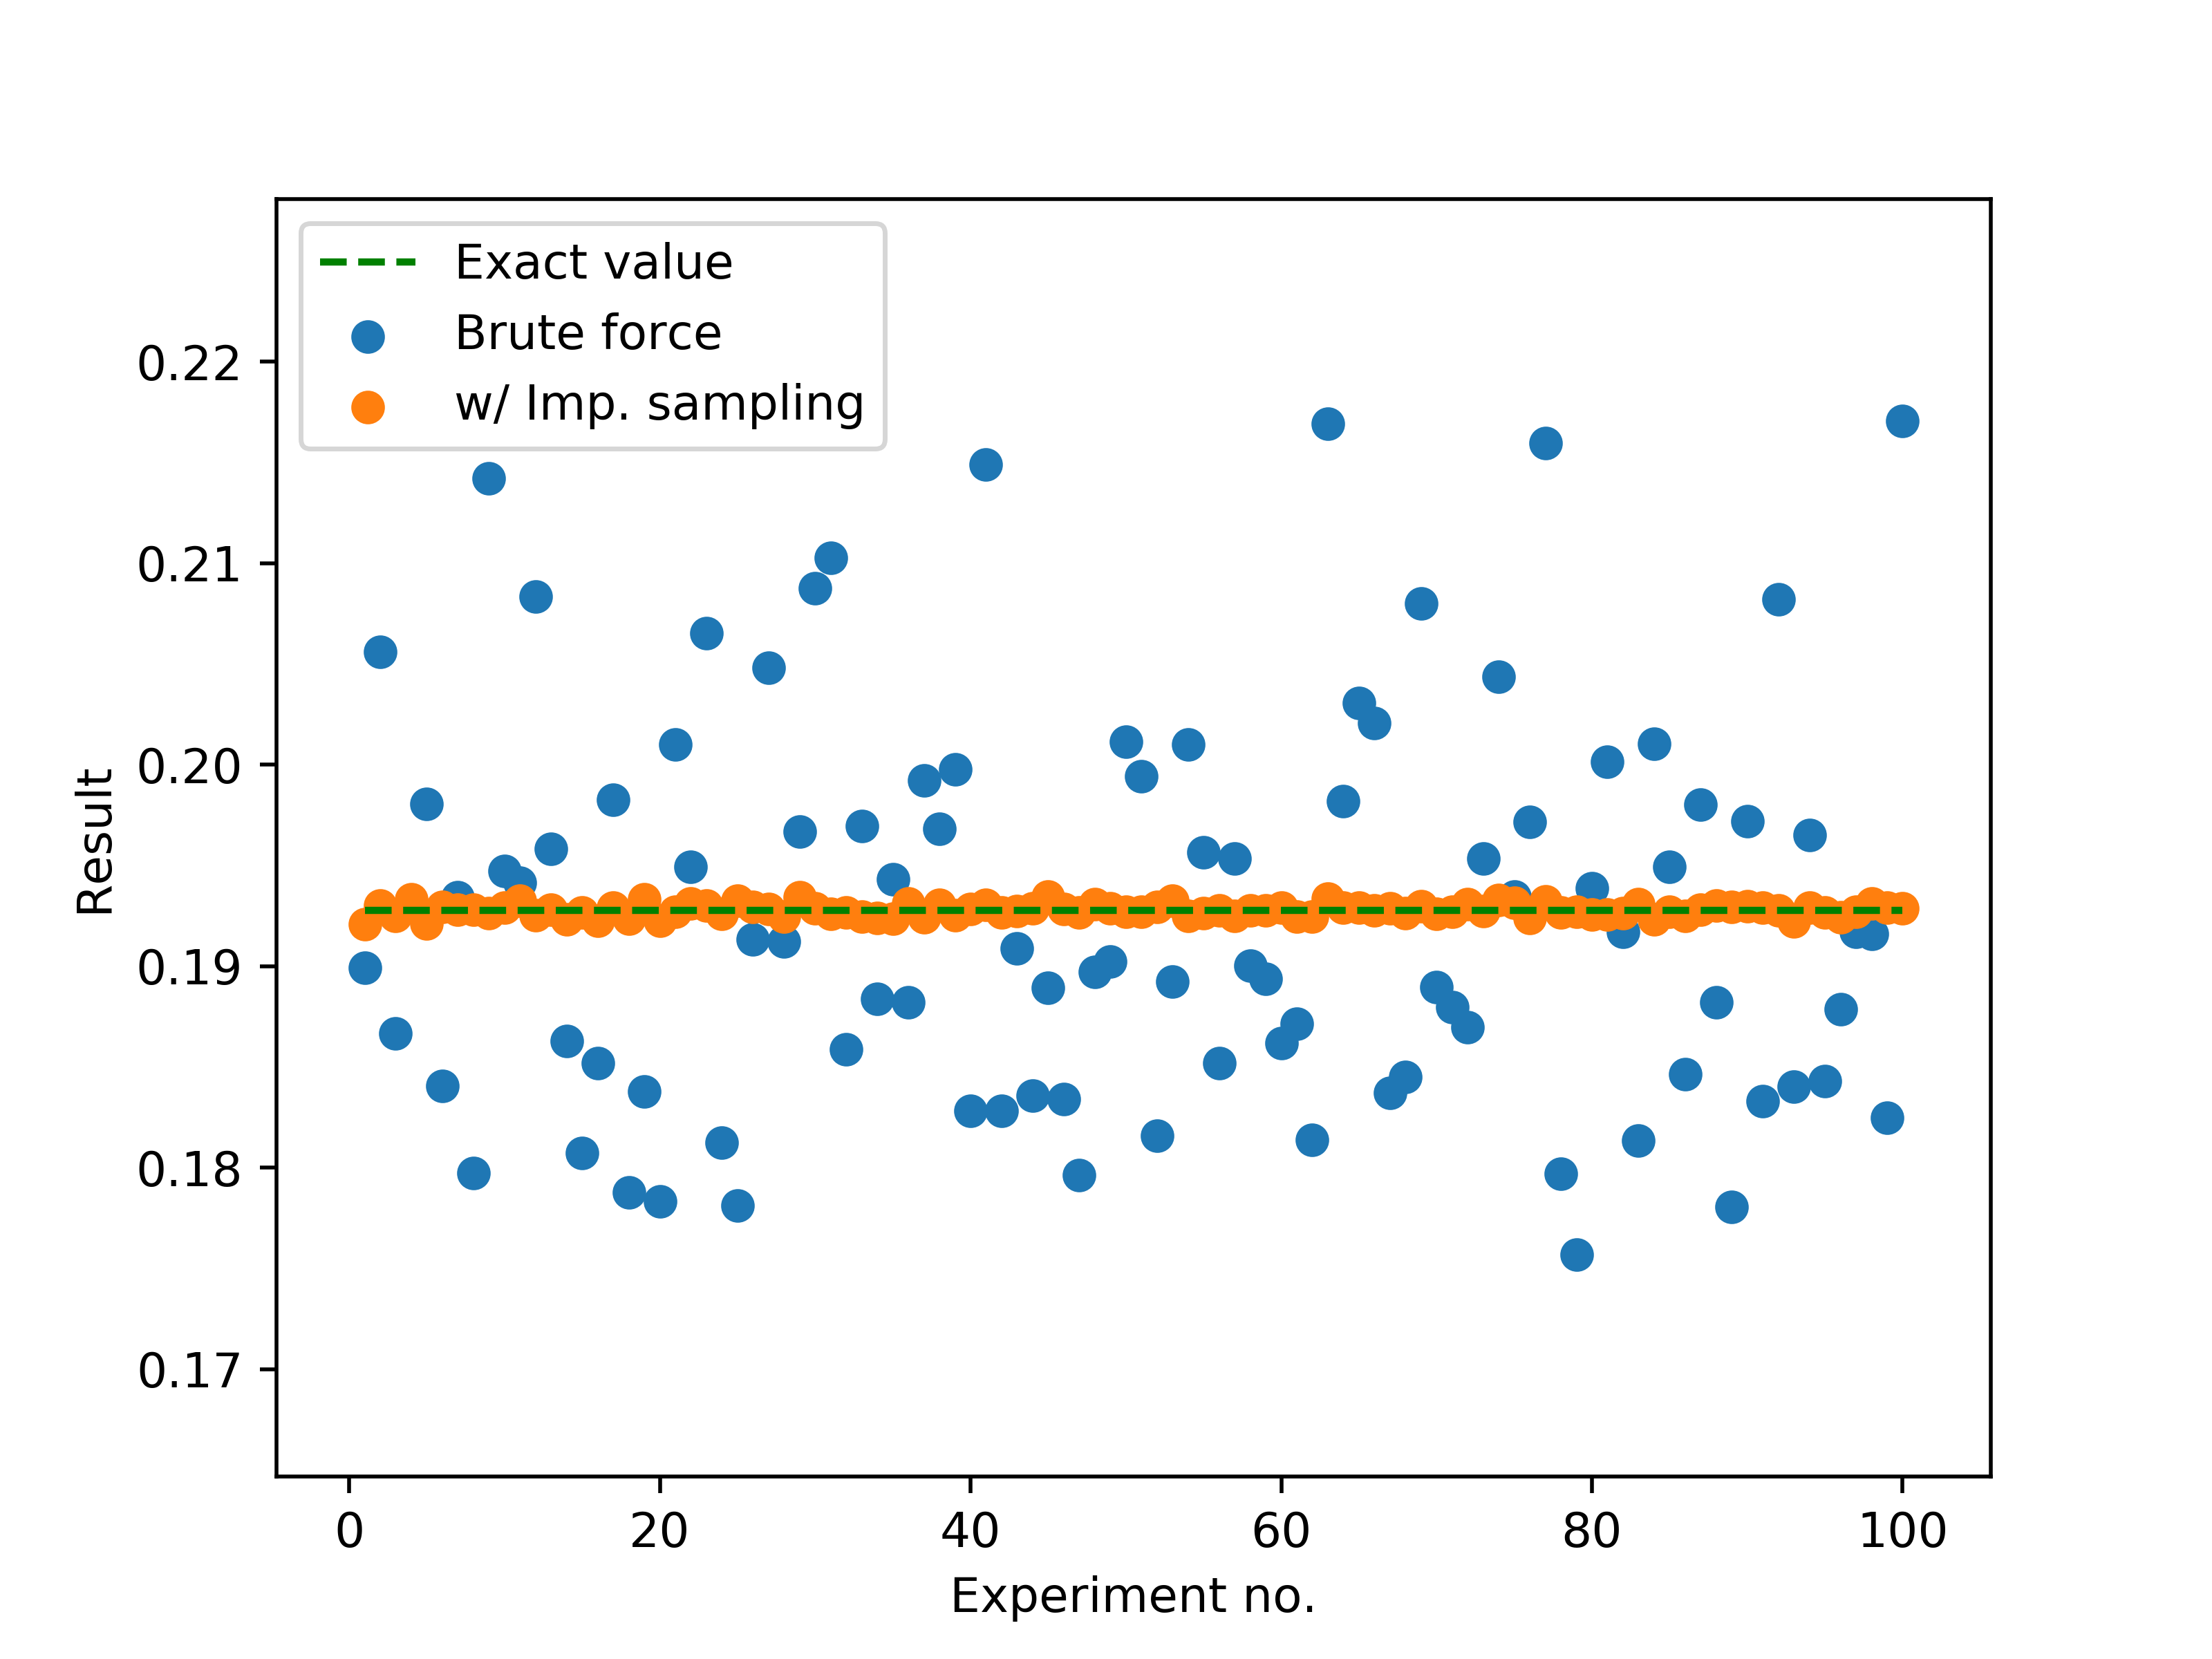
\includegraphics[width=0.8\textwidth]{bf_v_impsamp.png}
    \caption{A scatter plot of the result of 100 Monte Carlo experiments with $n=10^8$ iterations. }
    \label{fig:100_exps}
\end{figure}


\subsection{Parallelization}

Due to (comparatively) lack of experience with parallelization in the Julia programming language, the Monte Carlo integral approximation featuring importance sampling was implemented in C using MPI, while a serial version was also produced in C in order to compare the speedup from the parallelization. The calculations were done in the exact same way as in \ref{sec:mc_res}, with 100 iteration being run for each value of $n$. Since the granularity of the CPU timers in C are finite, it was decided that $n$-values under 1000 would not be included in the experiments. This time, since we are only interested in observing how parallelization affects the CPU time of the calculations, only this quantity will be presented. However, analysis of the results show that they did produce errors similar to those observed in the Julia implementation of the Monte Carlo methods. A table displaying the CPU time of the serial and parallel implementation, including the speedup gained from parallelization for each value of $log_{10}(n)$ is shown in figure \ref{tab:mc_parallel}.

\begin{table}[] \centering
\begin{tabular}{|l|l|l|l|l|l|l|}
\hline
\multicolumn{1}{|c|}{Time {[}ms{]}} & \multicolumn{6}{c|}{log10 n}                              \\ \hline
                                    & 3       & 4       & 5       & 6       & 7       & 8       \\ \hline
Serial                              & 0.00421 & 0.03548 & 0.36768 & 3.6012  & 35.777  & 362.46  \\ \hline
Parallel                            & 0.00163 & 0.0163  & 0.15718 & 1.58415 & 15.6419 & 155.243 \\ \hline
Speedup                             & 2.58282 & 2.17669 & 2.33923 & 2.27327 & 2.28726 & 2.33479 \\ \hline
\end{tabular}
\caption{A table showing the CPU time used for Monte Carlo integration with importance sampling. The n-values are how many sampling were performed. These results were produced in C, and parallelized with MPI.}
\label{tab:mc_parallel}
\end{table}




\section{Analysis}

From figure \ref{fig:legendre_all}, we see that the error of the approximated integral is high for larger values of $\lambda$. This is to be expected, as we saw in figure \ref{fig:lambda}, any values of $x>3$ will not contribute significantly to the area we are trying to approximate. When we are increasing $\lambda$, we are increasing the interval at which we are evaluating the function. Therefore, higher $\lambda$ will result in evaluating the function mostly in places where it is very close to $0$, which will give us a poor estimate of the total area under the graph.  The results of the integral approximation using Legendre polynomials shows us that the the best result (lowest error) was produced for $N = 27$ and $N=29$, both with $\lambda = 3$, with an error of $10^{-2.4} \approx 0.4\%$. However, with $\lambda = 2$, we were able to produce a similar result with $N=19$, this time with an error of $\approx 0.5\%$. While the most important aspect of a numerical integration is often to get the error a small as possible, one has to consider the numerical cost of the computations. In the case of the six-dimensional integral studied in this experiment, the Gaussian Quadrature scales with $O(N) \propto 10^6$, which means that a small increase in $N$ will lead to a substantial increase in the CPU time. Therefore, choosing the result from the experiment with $N=19$ and $\lambda = 2$ might be the best action, as you have to perform $10^{10}$ fewer iterations while still producing a result with an error that is only $0.3\%$ larger than for $N=29$. In the contour plot of the error (figure \ref{fig:legendre_odd}) we see that the error fluctuates between higher and lower values for odd $N$-point integrations. The reason for this is due to the fact that since the abscissas (the points at which we evaluate the function) are defined by the roots of the $N$th polynomial, the odd $N$-point integration will produce abscissas at $x=0$ since the odd polynomials all go through the origin. In order to avoid the singularity where $|\bold{r}_1 - \bold{r}_2| \approx 0$, as this would have caused division by zero and overflow, it was necessary to skip the contribution of the integral from the abscissas which resulted in this. Since the function, in Cartesian coordinates, is symmetrical around $\bold{r} = 0$, the abscissas generated by odd polynomials would always produce an abscissa at $0$, which again means we were forced to skip this result, resulting in a substantial loss in the contribution to the integral approximation. This issue is not an issue we observed when implementing the improved Gaussian quadrature method using Laguerre polynomials. As we see in the top right plot in figure \ref{fig:laguerre_legendre}, the result jumps extensively with Legendre polynomials for lower values of odd and even $N$, since most of the contribution of the area comes from the root at $\bold{r} = 0$. However, for the Legendre polynomials, we see that the integral approximation starts at $\approx 0$ for small $N$, before starting to rapidly approach the exact value as the polynomial degree is increased. From $N = 11$ to $N=13$, we see that the result actually crosses the exact value, and starts producing approximations that are higher than the analytical solution. We see this also in the plot of the error. The error produced by both the odd Legendre polynomials and Laguerre polynomials goes down as $N$ is increased, Laguerre has a much steeper negative slope, and reaches a minimum, before increasing again and flattening out as $N$ is further increased. The most important result here is that the Laguerre implementation not only produced a better error estimate than Legendre (Laguerre produced a minimum error of $\approx 0.3\%$, while Legendre had a minimum of $\approx 0.4 \%$), but it also reached this minimum at $N = 12$, while the Legendre implementation did not achieve its minimum error of $10^{-2.4}$ until $N=27$. With this in mind, we can turn our attention to the bottom plot in figure \ref{fig:laguerre_legendre}, showing the time usage of of the Legendre and Laguerre algorithms. Here we observe that both methods have a similar slope. However, for $N \geq 4$, the Laguerre method has a higher CPU time usage than the Legendre method. The reason for this is most likely due to having to call the function in spherical coordinates, which itself requires multiple calls to sine- and cosine-functions, functions that can be computationally expensive. One way to potentially circumvent this, since we are calculating many of the values multiple times, is to precalculate all the sine- and cosine values, stores these in arrays and look them up for each iteration. Nevertheless, the general purpose of the improved Gaussian quadrature method is observed in these results; by not having to approximate $\lambda$, we are able to produce better results with fewer iterations, as the integral approximation converges significantly faster when applying Laguerre polynomials rather than Legendre. 

In figure \ref{fig:montecarlo} we see the results of the Monte Carlo simulations. In the top right plot we see that the error of both the brute force method and the method implemented with importance sampling produces produce a better result as the number of iterations is increased. This is observed in that the error of the result decreases, in addition to the standard deviation. As we saw in in the derivation of the Monte Carlo integration method, this is the behaviour we would expect. With a larger number of randomly generated samples, we are able are evaluating the function at more parameters that are inside the domain of integration, giving us a better estimate of the area. While both methods improved in accuracy with a higher value of $n$, it was observed that the improved method featuring importance sampling with the exponential distribution produced significantly better results for smaller values of $n$. We see that for $n=10$, the improved method produced an error which was almost $100$ times smaller than the equivalent produced by the brute force method. While $n=10$ much too small of a number of iterations to produce accurate results, this visualizes the impact of choosing a good probability distribution function. As $n$ was increased, the same trend continued; the brute force method required approximately $10^2$ more steps than the improved implementation in order to produce similar results. This was also observed for the standard deviation of the results, which again is line with that we saw in \ref{eq:sigma_samp}. It should be noted that the mean error does not necessarily give a good estimation of the accuracy of the result, especially when using the brute force method. This is visualized in figure \ref{fig:100_exps}. In this figure we see a scatter plot of the results of 100 experiments of the brute force and improved method. We see that the brute force method varies significantly from experiment to experiment, while the method with importance sampling remains much more constant and close to the exact analytical solution throughout the experiments. Using the uniform distribution with $10^8$ iterations produces results that vary significantly, indicating a large standard deviation and variance of the model. Looking a the CPU time for both methods, we see that the improved method requires more CPU hours than the brute force implementation. This is equivalent with the results from the Quadrature methods; the improved methods are computationally more expensive, but they produce better results with fewer iterations. When comparing the improved quadrature method with the improved Monte Carlo method, we see that the best result from both methods produced errors of, respectively, $0.3 \%$ and $0.03\%$, while requiring a CPU time of $\approx 0.8$ and $200$ seconds. While this is a drastic difference, it must be noted that the Gaussian quadrature method with Laguerre polynomials scales with the dimensionality of the integral, which in this case was 6, while the Monte Carlo method does not increase in significant complexity as the integral dimension is increased. This means that while the Laguerre method required 2500 times less CPU time than Monte Carlo to produce an a respectable error, it would have required thousands of times this CPU time to produce an error of the same magnitude as the smallest error from the improved Monte Carlo method. This is due to the poor scalability of the Quadrature methods for higher dimensional integrals, and the gentle slope of the error as a function of $N$, as seen in the top left plot in figure \ref{fig:laguerre_legendre}. 


The parallel implementation of the improved Monte Carlo method produced the results displayed in table \ref{fig:montecarlo}. The program was run on hardware with 4 CPU cores, which implies that the ideal speedup should be 4. However, as we see in the results, the average speedup gained over all $n$-values is approximately $2.3$. The reason for this deviation can be due to a number of factors such as; lack of focus on optimizing the code, other programs using CPU power while the code was running, repeated calls to computationally expensive trigonometric functions which can take different amount of time depending on the number to evaluate. While there are most likely more parameters that affect the speedup of the parallel implementation, these potential causes all point to the same problem; the workers doing different amount of work. Nevertheless, it was observed that the parallelization of the Monte Carlo simulation was trivial task which did not require any rewriting of the main functions to evaluate. 

 \section{Conclusion}

In these experiments we have seen how different methods of evaluating numerical integrals affect both the accuracy of the result, and the CPU time required to compute them. It was shown that the Gaussian quadrature method using Legendre polynomials produced relatively accurate results, but required many iterations due to the high-dimensionality of the integral. Meanwhile, using Laguerre polynomials, we were able to produce a slightly better result using significantly fewer iterations, which. Therefore, despite the higher CPU time of the Laguerre method, we can conclude that it is a better model for approximation this specific integral. Meanwhile, using Monte Carlo integration methods, even more accurate results were produced. Using a uniform probability distribution for generating random numbers, an error close to that with Gaussian quadrature was observed. However, this was the mean error of several experiments, and further inspection of the results from each experiment revealed that the brute force Monte Carlo method was not a good approximation to the integral, as the result varied largely with each experiment. The improved method featuring important sampling proved to be superior to the brute force method, due to the sampling of parameters that contribute more to the area which we are trying to approximate. In fact, this method produced errors up to 30 times smaller for the same number of iterations, and had a significantly smaller variance in its results, visualizing the importance of using an appropriate probability density function when applying Monte Carlo methods for approximating integrals. At the same time, we observed one of the other strengths of Monte Carlo integration; its independence on the dimensionality of the integral. While a six-dimensional integral is not necessarily significant when compared to many modern physical problems, the Gaussian quadrature methods suffered in attempting to reduce the resulting error by a significant amount due to their scaling with the dimensionality. The Monte Carlo methods, on the other hand displayed a much stronger flexibility to reduce its error by increasing the number of iterations. In order to observe this difference between the quadrature and Monte Carlo methods more closely, one could make a figure showing the error per CPU time, which would give a clear overview of the scalability of both methods. Finally, we observed how the Monte Carlo methods can easily be parallelized as they feature independent looped operations. While we did not achieve the ideal speedup, for the simplicity of the implementation it can be concluded that parallelizing a Monte Carlo simulation should always be done when possible. In conclusion, Gaussian quadrature is potentially a good candidate for evaluating numerical integral of lower order, as a Monte Carlo integral would still require many iterations before producing satisfactory results. However, for high-dimensional integrals, Monte Carlo methods, due to their high scalability and ease of parallelization, should be strongly considered. 


\printbibliography
\end{document}
